\chapter{SLAM solution}  \label{chap::solution}
{\it \centering This chapter focusses exclusively on the solution to the impact-based SLAM problem. A modified version of the particle filter-SLAM algorithm will be developed to suit rectilinear environments, and the problem is extended to multiple robots for map-merging. Simulation results support the developed algorithm for both single robot and multiple robot-SLAM.}

\section{Factored representation} \label{sec::factpf}
In particle filter-SLAM, the uncertainty of robot pose is represented by a particle set (see Figure~\ref{robot_wall}) rather than a smooth parametric Gaussian as in EKF-SLAM. This representation has great advantages of representing any arbitrary multi-modal distribution, and they can be easily propagated through any probabilistic robot motion models.

However, there are downsides to implementing particle filter for SLAM due to a key reason. The number of particles scales exponentially with the dimension of the state space which restrict the use of particle filters to low-dimensional estimation and tracking problems. A suitable representation of particle filter towards the SLAM problem would be essential for an accurate SLAM solution. As discussed in Section~\ref{sec::pfslam}, the conditional independence property of the mapping problem given the robot trajectory is a key structure which can be exploited. This structural property in SLAM or any probabilistic problem that factorizes a joint distribution to conditional distributions is \textit{Rao-Blackwellization}.

Appendix~\ref{chap::rbpf} will provide a detailed proof of the conditional independence property in SLAM posterior and the exact nature of the factorization. Under this structure, cross-correlations between the landmarks introduced by the robot path uncertainty need not be maintained, and in the case of structured environments, explicit constraints are incorporated through \acs{CI} technique for ensuring consistency in estimation. The SLAM algorithms in future will utilize the conditional independence property for efficient computation of the posterior.

\section{Particle filter-SLAM}

Using the factored representation of the SLAM posterior, the SLAM solution can be obtained with linear time complexity in the number of landmarks, and the accuracy of obtained solution is proportional to the size of the particles. The particle filter-SLAM algorithm is simple and intuitive and a detailed algorithm is provided at each and every step.

Before delving into an algorithm, inclusion of data association into the SLAM posterior has to be discussed. The previous examples and illustrations assumed that data association is known, which is not the usual in SLAM. The general SLAM posterior is,
\begin{equation}
p(s_{1:t},m,c_{1:t}|z_{1:t},u_{1:t}),
\end{equation}  
where the it can be factorized through Bayes' product rule,
\begin{equation}
p(s_{1:t},m,c_{1:t}|z_{1:t},u_{1:t}) = p(s_{1:t},m|z_{1:t},u_{1:t},c_{1:t})\cdot p(c_{1:t}|z_{1:t},u_{1:t}).
\label{eq_slprod}
\end{equation}

The first term of the product is same as the old SLAM posterior and the second term correspond to the data association conditioned upon the observations. The vector $c_{1:t}$ is a vector of correspondences where each component makes a correspondence between a feature and a measurement.

\begin{rem}
The second term of the product in Equation~\ref{eq_slprod} corresponds to the data association, conditioned on the observations but not on the robot path. This discrete prior distribution about landmarks is not available initially and has to be engineered according to the sensors and operating environment.
\end{rem}

The FastSLAM algorithm maintains the (first term of the product) posterior distribution as a set of samples where each particle in the sample set corresponds to the state vector. According to the conditioned distribution, the map has to be conditioned on the robot trajectory and the length of each particle will grow over time. However, the update equations in FastSLAM, as in Section \ref{sec::pfslam}, do not depend upon the entire trajectory but only upon the most recent pose. Hence, each particle needs to contain the most recent pose and a map of the environment.

Each particle in the particle set $Y_t=\left\lbrace Y_t^{[1]}, Y_t^{[2]}, \dots, Y_t^{[M]}\right\rbrace$ of size $M$ takes the form as in Equation~\ref{psf},
\begin{equation}
Y_t^{[k]}=\left\langle s_t^{[k]}, \mu_{1,t}^{[k]}, \Sigma_{1,t}^{[k]}, \dots, \mu_{N,t}^{[k]}, \Sigma_{N,t}^{[k]} \right\rangle
\end{equation}  

The $k^{\text{th}}$ particle contains the recent robot pose and a corresponding set of landmarks of size $N$ where landmark $i$ is described by mean $\mu_{i,t}^{[k]}$ and covariance $\Sigma_{i,t}^{[k]}$ at time $t$.

From the particle set, the particles are propagated or sampled from the probabilistic motion model and the corresponding step is called as the Prediction step. The particles are then updated using incoming set of measurements and resampled if necessary. A simple flowchart explaining the process involved in the FastSLAM algorithm is illustrated in Figure \ref{flow_fs}. 
\begin{figure}
\centering
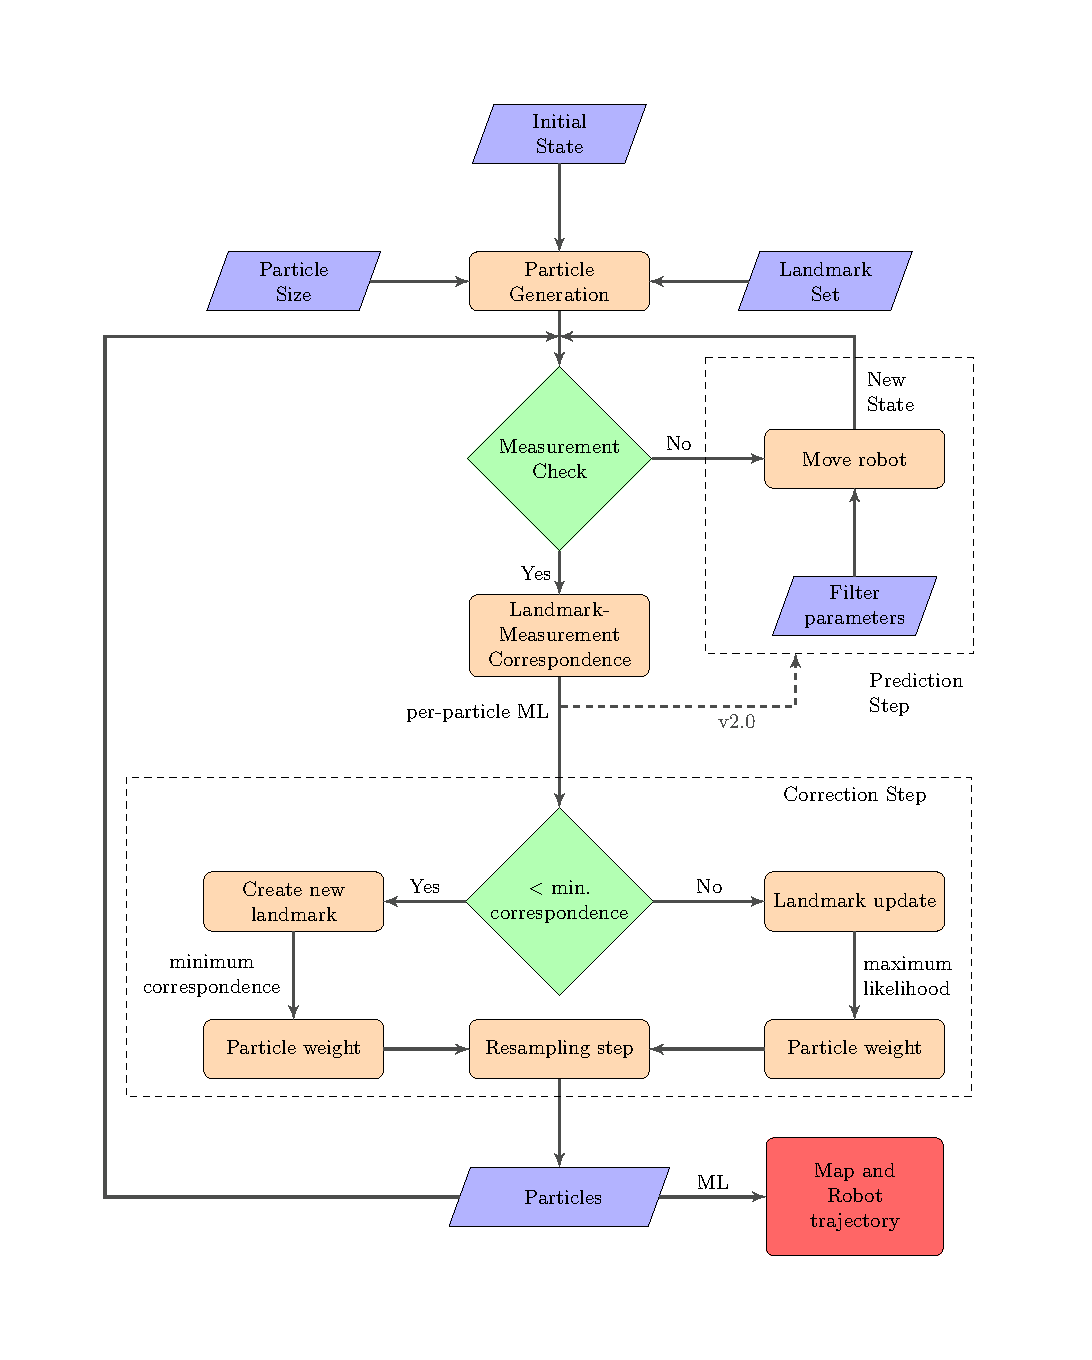
\includegraphics[scale=0.9]{./images/flow_fs}
\caption[A flowchart of particle filter-SLAM algorithm]{Particle filter-SLAM algorithm}
\label{flow_fs}
\end{figure}

The following sections will detail the individual steps involved in the algorithm.

\subsection{Particle generation}
Initially, a particle set of given size has to be created from a known distribution. The particles are either sampled from a Gaussian distribution whose mean correspond to the initial state of the robot and covariance corresponding the pose error or they are sampled from a prior particle distribution. In the SLAM scenario, the initial uncertainty is taken to be zero with no prior knowledge of landmarks.
\begin{equation}
Y_t^{[k]}=\left\langle s_0 \right\rangle
\end{equation}

As all the particles have the same initial state, the individual maps will also have the origin as the initial state.

\begin{rem}
The initial uncertainty in the position estimates (both robot and landmark) can also be non-zero, which ultimately converges to a stable solution. This can improve the initial diversity of the estimates and thereby ensuring a more consistent solution at the expense of time to converge to an accurate map. 
\end{rem}

\subsection{Prediction step} \label{sec::fastslam_pred}
The new state estimate is sampled from the old state using the probabilistic motion model and controls. The two motion models suitable to the SLAM scenario, along with the algorithm, are detailed in Section~\ref{sec::robotmodel}. 

The propagation of particles through the motion model has a linear time complexity $\mathcal{O}(M)$ and the new state estimate from each particle constitute to form a temporary particle set called as proposal distribution. This distribution takes the following form asymptotically,
\begin{equation}
p(s_t|u_t,s_{t-1})
\end{equation}

As the measurement likelihood is sparse or discrete with respect to the pose space in impact-based SLAM, the SLAM solution can be approximated to a Gaussian using Markov assumption for the measurement model. The current measurement depends upon the current robot pose and not on the previous set of poses. This assumption holds valid only since a complete state (refer Definition~\ref{def1}) is defined for the impact-based SLAM problem. Hence, the prediction step has to be repeated till a measurement is made available. The robot moves between the walls and a measurement is available only during a wall collision. As a result, the uncertainty in robot pose increases till a measurement is available.

The resulting motion model can be quite noisy and as said in the previous Chapter, this might result in a degeneracy problem. This arises when the robot motion is more noisy than the measurements. In the case of impact-based SLAM, the motion noise gets accumulated till a single measurement is made. Less particles will now be able to explain the new measurement and hence, particle diversity and consistency are lost during resampling(see Section~\ref{sec::conscorr} for more details). 

A favourable solution to the degeneracy problem is to modify the prediction step to include the measurements such that the proposal distribution is generated in accordance to incoming measurements \cite{montemerlo2007fastslam}. The modified proposal distribution can be written as,
\begin{equation}
p(s_t|s^{[k]}_{t-1},u_{1:t},z_{1:t},c_{1:t})
\end{equation}

In short, the variance propagation of measurements get included into the prediction step to obtain a better proposal distribution that can explain the incoming measurement. Hence, the proposal distribution remains closely same as the posterior distribution and particle diversity is retained. Appendix~\ref{mod_prop} gives a detailed proof of the modified proposal distribution.

For impact-based SLAM, the robot changes its heading direction (orientation in yaw axis) after every collision, which is encoded through a \acf{FSM} as shown in Figure~\ref{fsm4}. The FSM is modelled taking into account the exact nature of motion of robot between collisions. In forward motion, the robot can collide with the wall either on the left side or on the right side as shown in Figure~\ref{collision_ball}. This can restrict the size of FSM to two translational motion states (red shaded nodes) as in Figure~\ref{fsm4} where the left side represents the heading of robot towards a wall from left side and the other from right side. The rotation states describe the change in robot's orientation after every collision.

\begin{figure}
\centering
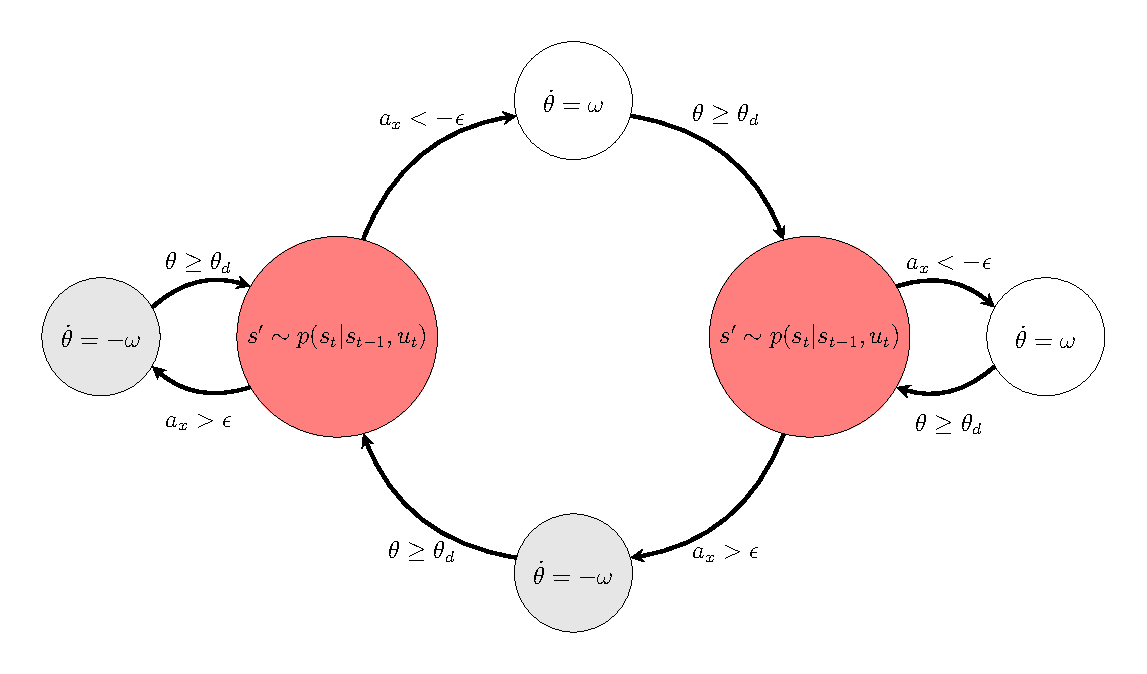
\includegraphics[scale=0.75]{./images/fsm4}
\caption[Finite State Machine model of robot-wall collisions]{Finite State Machine model of the robot motion between collisions. The red shaded nodes indicate the motion model of the robot. The gray and white shaded nodes indicate a specific control action on orientation corresponding to the sign of $a_x$. $\theta_d$ indicates the final desired angle through the function $T_i(\cdot)$ as in Equations~\ref{t1_orientation}~and~\ref{t2_orientation}.}
\label{fsm4}
\end{figure}

\begin{figure}
\centering
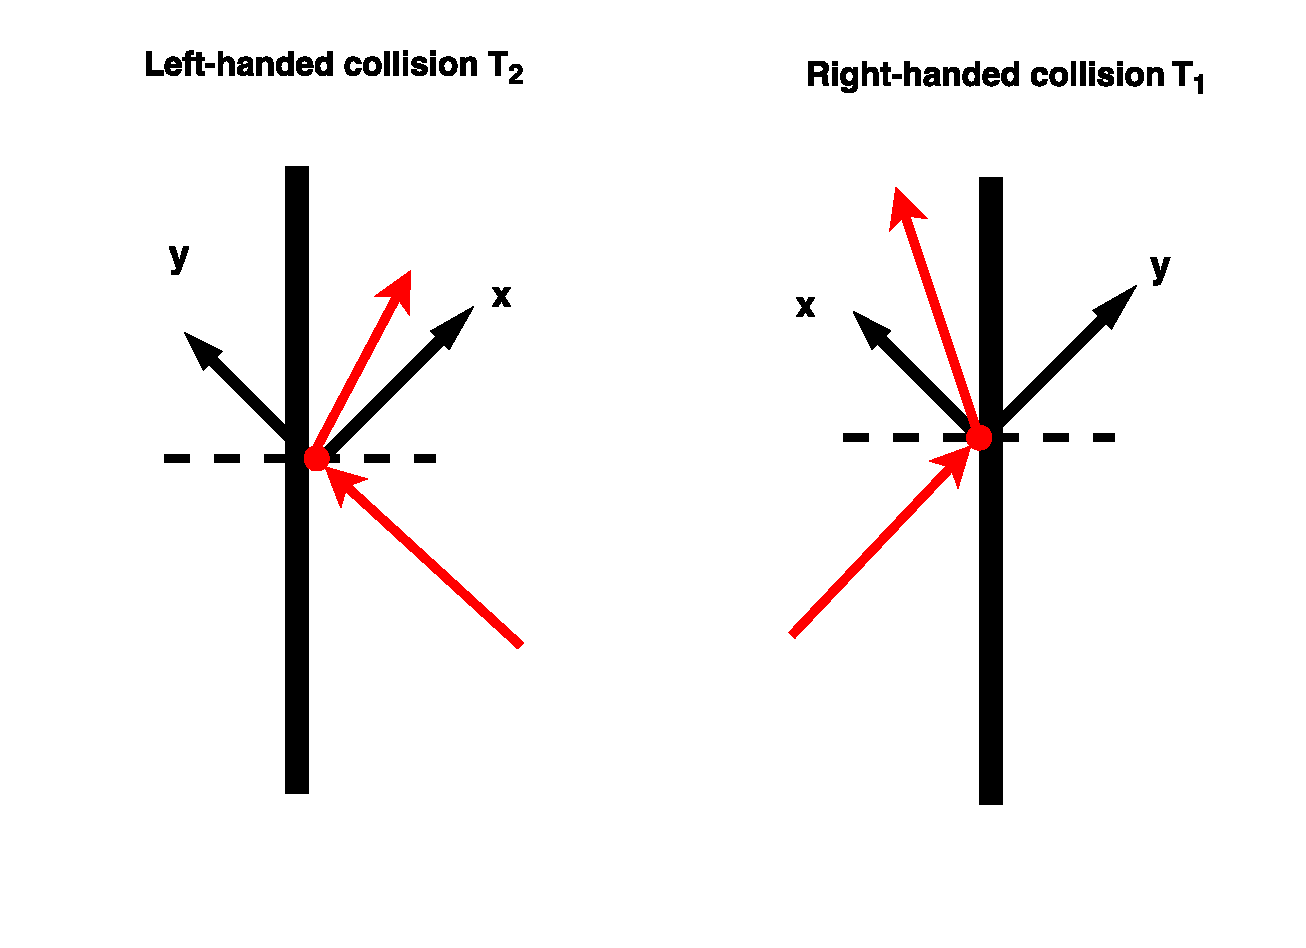
\includegraphics[scale=0.6]{./images/collision_ball}
\caption[Types of collision generation in impact-based SLAM]{Approach of robot towards a rectilinear wall restricts to two possible cases, left-handed collision and right-handed collision. The black arrows depict the local coordinate frame of the robot before collision and the red arrows depicts the robot motion. The ratio of change in impact force along the individual axis is used as collision measurement.}
\label{collision_ball}
\end{figure}

The underlying motion model used for the FSM in prediction step is the same unicycle model in Section~\ref{sec::robotmodel} as follows,
\begin{equation}
s'\sim p(s_t|s_{t-1},u_t)
\end{equation}

The change in robot's orientation depends upon the collision of the robot with the wall from the left or right hand side. With a coordinate frame is assigned to the robot, the forward motion of the robot is Y-axis and to the right is X-axis. As the collision detection is achieved through changes in the accelerometer values, the left-handed collision of the robot with a wall has negative acceleration on the X-axis while the right-handed collision of the robot with a wall has positive acceleration on the X-axis. This can be described through a change in orientation for the robot where the left-handed collision model is written as,
\begin{equation}
T_1(\theta,a_x)=\theta-\left(\pi-c\cdot\arctan\left(\frac{a_x}{a_y}\right)\right),
\label{t1_orientation}
\end{equation}
and the right-handed collision model as,
\begin{equation}
T_2(\theta,a_x)=\theta+\left(\pi-c\cdot\arctan\left(\frac{a_x}{a_y}\right)\right).
\label{t2_orientation}
\end{equation}

The constant $c$ is the reflection constant which varies according to the requirement of desired heading after a collision. For a reflective collision i.e., angle of incidence is same as angle of reflection, the value of $c$ is 2. The initial orientation $\theta$ in yaw axis of the robot is obtained from the IMU. Further details of Sphero robot motion after collision is detailed in Section~\ref{sec::single_slam}.  

\begin{rem}
The false positives in collision detection may arise from the positive acceleration in the forward direction. This can be avoided by considering only the positive acceleration hyperplane in collision detection, i.e., $a_y>0$.
\end{rem}

\subsection{Data Association}
The data association for the impact-based SLAM performs a landmark-measurement likelihood computation on a per-particle basis. Three key advantages with the per-particle data association are as follows,
\begin{itemize}
\item Multi-hypothesis data association is the robust form of data association till date.
\item Consistent landmark updates can be carried out on a per-particle basis since landmarks in a particle do not depend upon robot pose uncertainty as robot pose error is factored out.
\item Data association decisions can be revisited by removing particles which cannot explain incoming measurements and resampled with a particle which is consistent with new measurements. 
\end{itemize}

The association is sensitive to the source of uncertainty arising from the motion or measurement model. An increase in measurement noise can lead to a wrong association of a measurement to a landmark. This is because as the measurement uncertainty increases, the distribution of measurements from nearby landmarks start to substantially overlap. As a result, some landmarks get wrongly associated which might lead to a underestimation (spurious reduction) of covariance. This problem will have a minor impact on the SLAM solution, provided landmarks are not close by. However, the noise from the motion model will have a more drastic impact since higher uncertainty in the robot pose leads to a wide distribution of particles and the resulting per-particle data association will be quite different. This situation occurs in the impact-based SLAM problem where the motion noise gets accumulated between the sparse measurements. This problem in association can be reduced using the modified proposal distribution as mentioned in the previous section. 

Using the per-particle data association, the worst-case computational complexity involved in computing the likelihood is proportional to $\mathcal{O}(N\cdot n^3)$, where $N$ is the size of landmark set and $n$ is the dimension of output vector. This can be computationally intensive which can be reduced on an average case through a pruning process. The process prunes the landmark with orientations which are not in the field of view for the robot, which also contributes to finite nature of FSM in a rectilinear environment. In addition, geometric constraints can be added to improve the efficiency of association. One such geometric constraint is the feature pose of the same landmark. In the robot's view, feature orientation of 0~degree always come to the right of a feature with an orientation of 180~degrees with respect to the robot's frame.   
 
\begin{figure}
\begin{algorithm}[H]
\caption{Per-particle data association} \label{ppda}
\begin{algorithmic}[1]
\BState \textbf{Input}: $z_t$, $R_t$ , $Y_t$ and $m_{1:N}$
\For{each particle \Pisymbol{psy}{206} $Y_t$}
\State $l \gets \left[\,\right]$
\For{each landmark \Pisymbol{psy}{206} $m_{1:N}$}
\State compute expected measurement
\If {geometric constraint not satisfied} 
\State $l$.append(0)
\EndIf
\If {landmark in robot's view}
\State compute likelihood
\State $l$.append(likelihood)
\ElsIf {check similar features}
\State create feature if not present in landmark list
\State compute likelihood
\State $l$.append(likelihood)
\Else 
\State $l$.append(0)
\EndIf
\EndFor
\State \Return correspondence $\gets \text{max}(l)$
\EndFor
\end{algorithmic}
\end{algorithm}
\caption[Per-particle data association algorithm]{Per-particle data association is carried out using an incoming measurement $z_t$, measurement covariance $R_t$, particle set $Y_t$ and landmark set $m_{1:N}$.}
\end{figure}

In computing the measurement likelihood, correspondence was computed only from the set of point landmarks, and histogram information is not used. Similar to occupancy maps, histogram maps can be used for localizing the robot using the occupancy information. However, a sufficient amount of collision information along the wall is necessary to influence the localization. The use of histogram information (as a probability distribution) in data association will be more promising in situations where the rectilinear landmarks are more randomly placed.  

\subsection{Landmark update} \label{sec::land_update}
The data association step might provides a landmark identity once its correspondence with a measurement satisfies the compatibility test and it is found to be more likely than other landmarks. As the data association step is carried out on a per-particle basis, the corresponding landmark update is also carried similarly. The rest of the landmark set remain unchanged.

The landmark update stage is a part of the mapping problem, described through the posterior $p(m_l|s_t,u_{1:t},z_{1:t},c_{1:t})$. Expanding the term using Bayes' product,
\begin{equation}
p(m_l|s_t,u_{1:t},z_{1:t},c_{1:t})=\eta\,p(z_t|m_l,s_t,u_{1:t},z_{1:t-1},c_{1:t})\cdot p(m_l|s_t,u_{1:t},z_{1:t-1},c_{1:t}) 
\end{equation}

The first probabilistic term of the above product corresponds to the measurement model and is approximated as a Gaussian using EKF linearization. The second term is the landmark estimate conditioned on the particle pose which is equal to the mean and covariance estimates of the landmark maintained by a particle $\mathcal{N}\left(\mu^{[k]}_{l,t-1},\Sigma^{[k]}_{l,t-1}\right)$.
 
EKF uses a linear approximation of the measurement model $h(\cdot)$ which is obtained through a first order Taylor series expansion. According to the conditioned measurement distribution, each landmark update in a particle is carried out over a fixed robot pose. This property favours computation since the Jacobian over robot pose \lsymb{$G_{s^{[k]}_t}$}{Jacobian of measurement model over particle pose} in an EKF update is unnecessary. As a result, the Jacobian over the associated landmark \lsymb{$G_{m_{l,t}}$}{Jacobian of measurement model over landmark pose} is only calculated in the Taylor expansion. 
\begin{align}
\hat{z}_t &= h(s_t^{[k]},\mu^{[k]}_{l,t-1}) \\
G_{m_{l,t}} &= \nabla_{m_l} h(s_t=s_t^{[k]},m_l=\mu^{[k]}_{l,t-1}) \\
h(s_t,m_{l,t}) &\approx \hat{z}_t+G_{m_l}(m_{l,t}-\mu^{[k]}_{l,t-1})
\label{taylor_approx}
\end{align}

The mean of the Gaussian is approximated till the first order Taylor expansion and the covariance is assumed to be known initially. The derivative of the measurement function is defined everywhere except in cases where robot and wall orientation are the same (robot collides parallel to the wall) at the point of collision. This situation is not possible in impact-based SLAM using Sphero. The parametrization of a Gaussian measurement can be written as,
\begin{equation}
\mathcal{N}(\hat{z}_t+G_{m_l}(m_l-\mu^{[k]}_{l,t}),R_t)
\end{equation}

The mean and covariance of the associated landmark can now be computed using the standard EKF update equations.
\begin{align}
S_{l,t} &= G_{m_l}\Sigma^{[k]}_{m_{l,t-1}}G^T_{m_l}+R_t \label{ekf_update1}\\ 
K_t &= \Sigma_{m_{l,t-1}}G^T_{m_{l,t}}S^{-1}_{l,t} \\
\mu^{[k]}_{l,t} &= \mu^{[k]}_{l,t-1} + K_t\left(z_t-\hat{z}_t\right) \\
\Sigma^{[k]}_{l,t} &= \left(I-K_tG_{m_l}\right)\Sigma^{[k]}_{l,t-1} \label{ekf_update2}
\end{align}

The term \lsymb{$S_{l,t}$}{Innovation covariance} and $K_t$ represent the innovation covariance of landmark $l$ and Kalman gain at time $t$ respectively.

\subsubsection{Negative evidence}
A new histogram is created once a new landmark is detected. This histogram is maintained either as a probability distribution or as a simple histogram for encoding the collision information. In the case of a probability distribution, the histogram is defined as a uniform distribution, based on the prior assumption that the distribution of mass information is unknown. The probability mass propagates into the regions where collisions were detected and a multimodal distribution is generated as seen in Figure~\ref{ex24coll_10}.

With the histogram representation, negative information can be incorporated into the map. As the robot passes through the histogram axis in the map, a negative Gaussian information is added to the histogram as shown in Figure~\ref{ex24_coll15}. This information helps in pruning the histogram support. If the environment size is known prior, the histogram support can be made finite according to the environment size.

\subsection{Landmark initialization}
The landmark is initialized each time a new measurement is unable to explain all the landmarks in the landmark set or when the landmark set is empty. The data association step in the previous section assumed that all the landmarks were available prior.

The landmarks are initialized using the inverse measurement model, provided the measurement function (see Equation~\ref{measurement_eq}) is invertible. The inverse is ill-defined in a SLAM problem when a given measurement is unable to constrain the landmark state and multiple measurements are required (as in range-only or bearing-only SLAM). However, the measurement model of impact-based SLAM is invertible since the landmark pose at time $t$ is calculated through the conditioned robot pose, odometry and collision information at time $t$.
\begin{equation}
\mu^{[k]}_{l,t}=\begin{bmatrix}x_l \\ y_l \\ \psi_l
\end{bmatrix} = \begin{bmatrix}x^{[k]}_r \\ y^{[k]}_r \\ \psi^{[k]}_r+\arctan\left(\dfrac{a_x}{a_y}\right)\end{bmatrix}
\label{inv_measurement}
\end{equation}

The landmark pose $m_l$ is described as a vector of landmark position \lsymb{$(x_l,y_l)$}{XY-position of landmark} and orientation \gsymb{$\psi_l$}{Orientation of landmark}. Similarly, the robot pose for a particle $k$ is described as a vector of robot position \lsymb{$(x^{[k]}_r,y^{[k]}_r)$}{XY- position of $k^{\text{th}}$ particle pose} and orientation \gsymb{$\psi^{[k]}_r$}{Orientation of particle pose}. \lsymb{$a_x$}{Rate of acceleration along the X axis} and \lsymb{$a_y$}{Rate of acceleration along the Y axis} denote the rate of change in accelerometer data along the X and Y axes respectively.
\begin{rem}
The offset between the position of landmark and robot at the instant of collision varies by a constant factor. This factor should be taken into account for the resulting output map of SLAM. 
\end{rem}

As the measurement is obtained from a nonlinear model, a first order Taylor expansion (as in Equation~\ref{taylor_approx}) can reveal the Gaussian nature of the noise where the difference in the approximation is the error $e_t$,
\begin{equation}
e_t=z_t-\hat{z}_t-G_{m_l}(m_l-\mu^{[k]}_{l,t})
\end{equation}
and the Gaussian as,
\begin{equation}
\mathcal{N}:= \dfrac{\displaystyle 1}{\displaystyle \sqrt{\mathstrut|2\pi R_t|}}\exp\left(-\frac{1}{2}e_t^TR_t^{-1}e_t\right)
\label{exp_gaussian}
\end{equation}

The landmark covariance is obtained through the covariance bound of the $\chi^2$ distribution (see Definition~\ref{chi2_dis}). The measurement covariance propagation through the SLAM state space is obtained by projecting the measurement covariance into the landmark state space, which is equivalent to calculating the second differential of Equation~\ref{chi2_eq}. As the landmark is defined using inverse of the measurement model, the landmark covariance is the inverse of the measurement covariance propagation.

\begin{defn}
The $\chi^2$ distribution is the negative exponent of the Gaussian $\mathcal{N}$ as shown below,
\begin{equation}
\chi^2 := \left(z_t-\hat{z}_t-G_{m_l}(m_l-\mu^{[k]}_{l,t})\right)^TR_t^{-1}\left(z_t-\hat{z}_t-G_{m_l}(m_l-\mu^{[k]}_{l,t})\right).
\label{chi2_eq}
\end{equation}
\label{chi2_dis}
\end{defn}

As a result, the mean $\mu^{[k]}_{l,t}$ is obtained through the inverse of measurement model (Equation~\ref{inv_measurement}) and the covariance $\Sigma^{[k]}_{l,t}$ is obtained from the second differential of the Equation~\ref{chi2_eq} and taking the inverse since an invertible measurement is used to define a new landmark.

\begin{align}
\mu^{[k]}_{l,t} &= h^{-1}\left(s^{[k]}_t,z_t\right) \label{landmark_init1}\\
\Sigma^{[k]}_{l,t} &= \left(G_{m_l}^TR_t^{-1}G_{m_l}\right)^{-1} \label{landmark_init2}
\end{align}

As the measurement model has a diagonal symmetry where each state depends upon only few variables, the Jacobian with respect to landmark states will be diagonal as well, which gives way to a computationally efficient approach to a initialize a new landmark.

A faster initialization (on average time efficiency) procedure can be performed for covariance computation for all the landmarks by assuming a spherical initial covariance. The magnitude of this uncertainty has to be computed by conducting trials on various values of magnitude through an eigenvalue decomposition (average computational complexity is $\mathcal{O}(n^3)$) to recover the largest magnitude. This approach is however numerically unstable since the uncertainty involved in the update process is high.

In addition to the landmark initialization using mean and covariance which is common to histogram and point landmark representation, a histogram has to be created with a finite support especially for a histogram map. The length of the support depends upon the boundary length or can be set arbitrarily and pruned later. Example~\ref{exmp_tree} gives a detailed representation of defining a new landmark with a histogram. 

\begin{exmp}{\it Consider a simple 2-D rectilinear environment as shown in Figure~\ref{rect_world}, with a robot doing impact-based SLAM. The walls are numbered from 1 to 6 in red color and landmarks are initialized using EKFs as in Equations~\ref{landmark_init1}~and~\ref{landmark_init2}.}
\begin{figure}
\centering
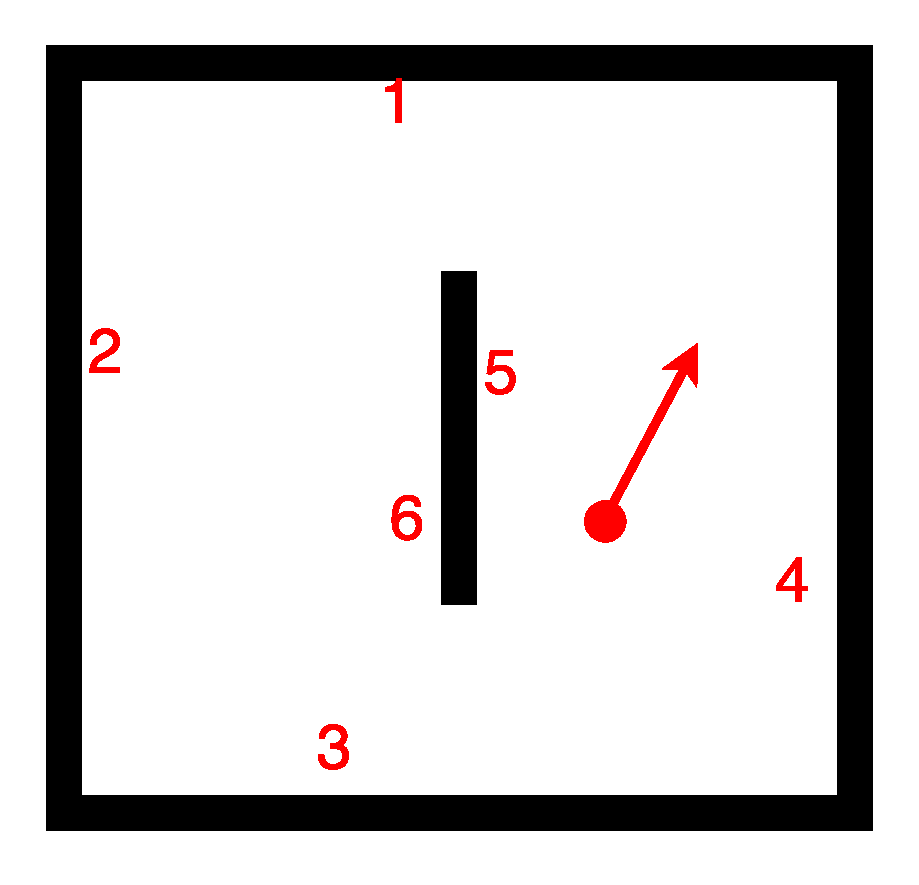
\includegraphics[scale=0.4]{./images/add_landmark}
\caption[A sample rectilinear world]{A simple rectilinear world}
\label{rect_world}
\end{figure}
\begin{figure}
\centering
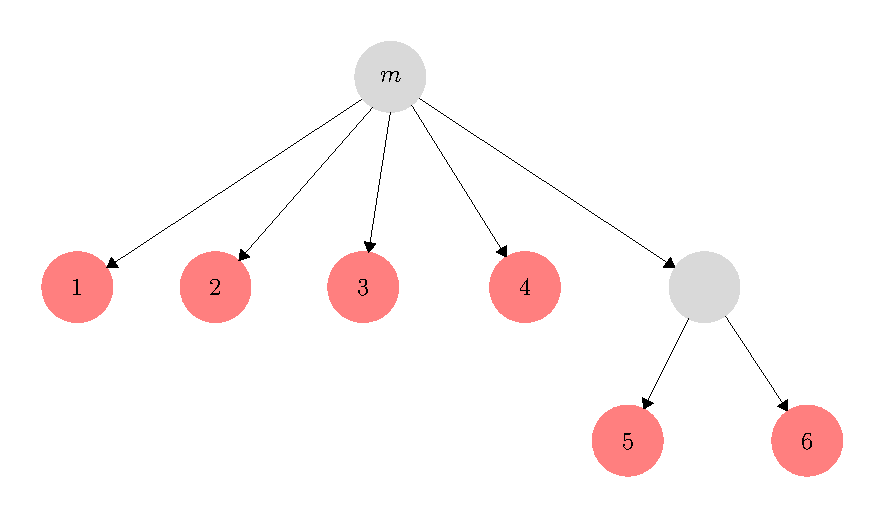
\includegraphics[scale=1]{./images/fsm7}
\caption[A tree data structure for landmark representation]{A tree data structure for landmark representation in Example~\ref{exmp_tree}}
\label{tree_landmark}
\end{figure}
\label{exmp_tree}
\end{exmp}
The landmarks are defined and propagated using a tree representation which is efficient in access and storage. The map is created as a root node or a pseudo-node to the tree. The individual landmarks are appended as a leaf node to the tree. A simple geometrical structure is exploited to reduce the number of leaf nodes in the tree. Walls 1 to 4 can be regarded as a landmark and a histogram has to be created for each of them to encode the collision information. However, for walls 5 and 6 represent the same wall back-to-back and a single landmark pose is sufficient to maintain. Hence, walls 5 and 6 are regarded as features of the same landmark and a single histogram is sufficient. The representation is illustrated in Figure~\ref{tree_landmark}.
\hfill $\square$

\subsection{Importance resampling} \label{sec::fastslam_resample}
After the particles are updated using an incoming measurement based on the maximum correspondence likelihood, the SLAM algorithm is not yet done. The mapping part of SLAM has been completed for the entire particle set where the localization (robot pose in particle) is found to influence the map. According to the SLAM definition, the robot must able to build a map using its pose as well as localize itself within the built map, or in simple words in relevance to the context, the localization and mapping must improvise each other. Hence, the mapping part of SLAM has to influence the robot pose or equivalently, the particle set to be distributed according to the posterior belief.

An improvised set of particles are drawn for the next iteration through resampling. Each particle is weighted in proportion to the likelihood of the measurements using the sensor model (refer Section~\ref{sec::pfslam}),
\begin{equation}
p(z_t|s_t,m),
\end{equation} 
where this likelihood computation is done in the data association step (refer Appendix~\ref{mod_prop} for importance weight calculation for the case of modified proposal distribution). This technique in particle filters is called \acf{SIR}. As the likelihood of measurements gets higher, the particles can explain the incoming measurements well, and with a higher probability they are drawn for the next iteration. Hence, the particles with an accurate robot pose are more likely to retain in the distribution and localization is achieved through the mapping process with the help of resampling.

After few resampling steps, the particles might lose diversity and there might be a single particle that got duplicated several times. This is a crucial problem in particle filters called as the degeneracy problem. This has a huge impact in the consistency of SLAM solution (as explained in Section~\ref{sec::conscorr}) since particles cannot revisit their past data association history. Usually, consistency is ensured by resampling particles that can explain the measurements which holds true only for systems which exhibit forgetting of past estimation errors. This is not the case for SLAM since the past pose error plays a key role through landmark-pose correlations for obtaining a consistent solution. The inconsistency arises when a particle lost through resampling, the corresponding pose and a entire map hypothesis gets lost. The past pose information gets lost along with the corresponding map estimate and might result in poor loop closures. Greater diversity in a particle set ensures the SLAM algorithm to revisit their past associations and prune them (by assigning low weights) if necessary.

In such a case, an adaptive resampling technique \cite{grisetti2005improving} can be adopted where a criterion can be established about when to perform a resampling step. The criterion has to find the \textit{effective number} of particles $N_{\text{eff}}$ which estimates how well the current set of particles represents the posterior distribution. This criterion can be computed as follows,
\begin{equation}
N_{\text{eff}}=\frac{\displaystyle 1}{\displaystyle \sum_{k=1}^N\left(w^{[k]}\right)^2}
\end{equation}     

The intuition behind the use of $N_{\text{eff}}$ is simple as follows. If the particles are drawn from the true posterior, the variance in the weights achieves a minimum and grows as the approximation of true posterior deviates. This measure of dispersion can inform when a resampling step can be performed. As $N_{\text{eff}}$ falls below a suitable threshold (usually around $N/2$), the particles are resampled. As a result, particle diversity is ensured by maintaining a good set of particles or hypothesis.

\section{Simulation Results}
This section supports the SLAM algorithm developed in the previous section with simulation results in the form of graphs and output map. A two dimensional world, as shown in Figure~\ref{sample_world}, is considered for the simulation with a ball robot modelled using unicycle-FSM model.
\begin{figure}
\centering
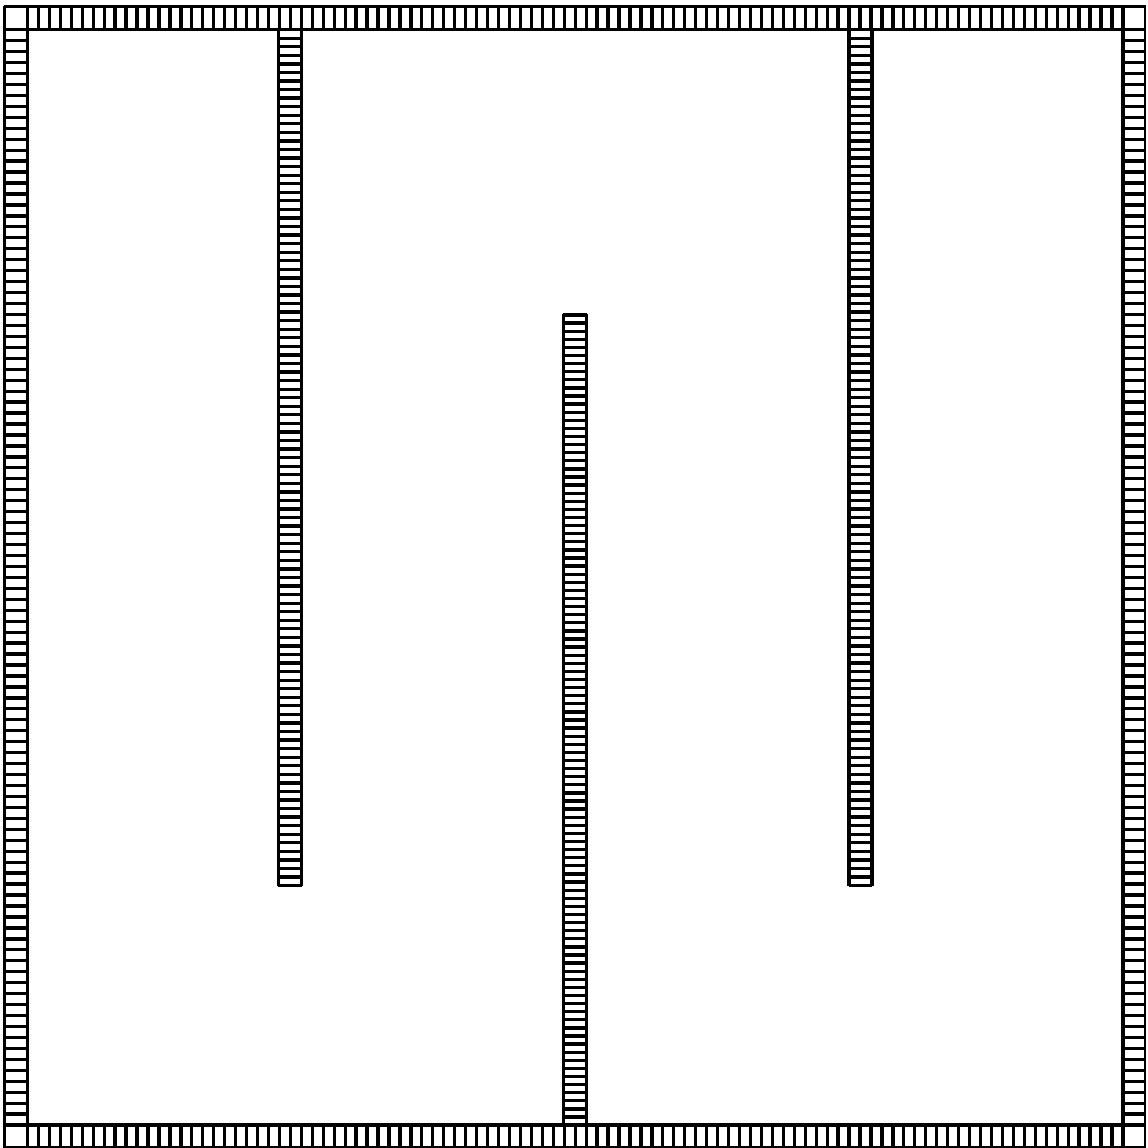
\includegraphics[scale=0.4]{./images/sample_world}
\caption[Rectilinear world as a simulation environment]{Sample world for the simulation environment}
\label{sample_world}
\end{figure}

The odometry is obtained using the accelerometer and gyroscope through dead-reckoning. In the ideal case, the position information provided by the robot should be same as the robot's actual position, provided there are no slip between the robot and the ground. However, the odometry information is subject to significant drift which has to be accounted in the simulation scenario. Since the collision information is also obtained from the robot's IMU, it is also subject to drift. Figure~\ref{odom_simulation} shows the drift in the odometry from the true position, which is considered in the simulation. The drift is obtained through addition of Gaussian noise information where Figure~\ref{odom_error} shows a higher translation drift than rotational drift while Figure~\ref{odom_error2} shows a higher rotational drift than translational drift.
\begin{figure}
\centering
\begin{subfigure}{0.47\textwidth}
\centering
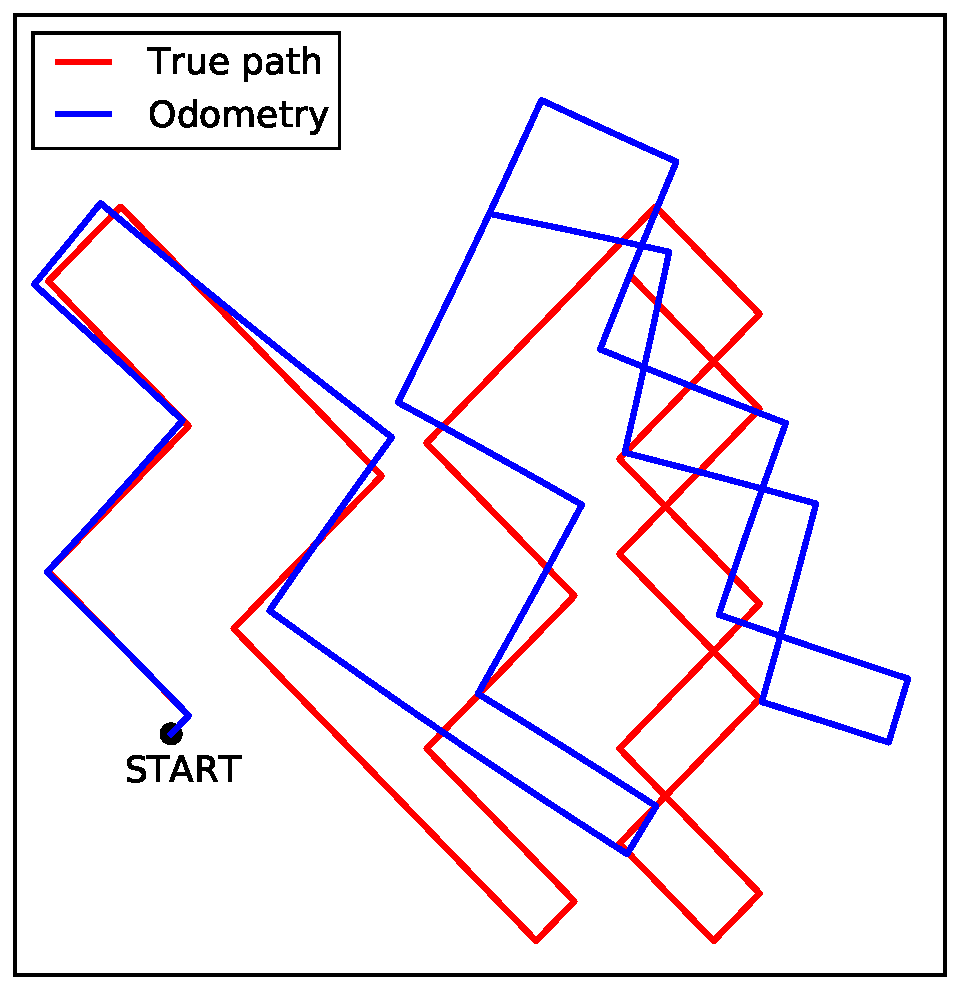
\includegraphics[scale=0.45]{./images/odom_error}
\caption{}
\label{odom_error}
\end{subfigure}
\begin{subfigure}{0.47\textwidth}
\centering
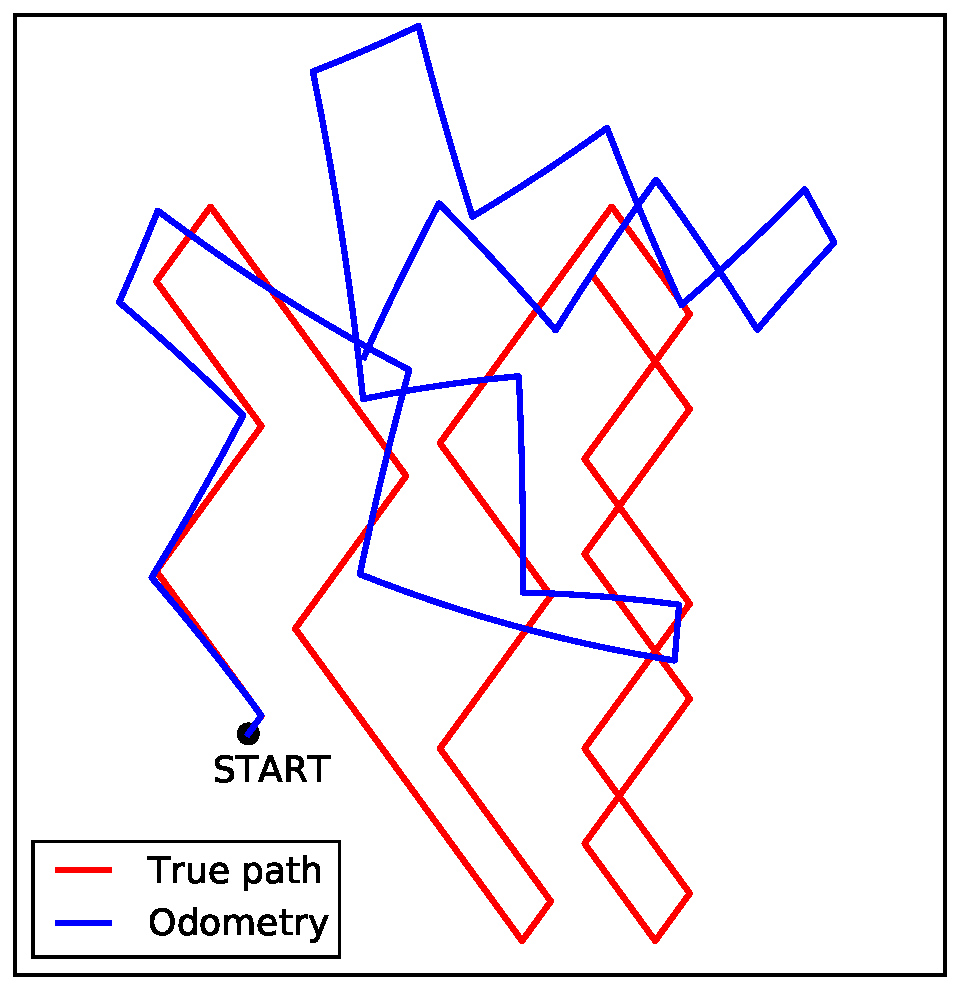
\includegraphics[scale=0.45]{./images/odom_error2}
\caption{}
\label{odom_error2}
\end{subfigure}
\caption[Odometry information in simulation]{Odometry information for the two possible cases of error- translational and rotational. The left figure has a higher translation error while the right figure has a higher rotational error.}
\label{odom_simulation}
\end{figure} 

The noise in the odometry and collision data have to filtered out against a model using a suitable estimator. The previous sections in this Chapter laid out a suitable algorithm for the impact-based SLAM where the odometry and collision data are filtered to obtain a suitable map of the environment along with the current robot pose (or the entire trajectory). A particle filter is initialized with $M=10$ particles with the same initial state. The initial pose is trivially taken to be as the origin unless an exact pose is needed to plot the map on a figure window. The initial uncertainty is taken to be very small (zero if possible) to get a more consistent map. The size of the particle set $M$ may vary depending upon the noise covariance of the measurement, including the odometry.

In the prediction, a new set of particles are drawn from the (modified) proposal distribution. In the case of a modified proposal distribution, the particles are drawn from the modified proposal only when a measurement is made available and for rest of the time, the old proposal distribution is used.

As discussed earlier, suitable environment representations for impact-based SLAM are point landmarks and histogram landmarks.
\begin{rem}
The most suitable environment representation for the SLAM problem depends upon the sensor used and the operating environment. For example, in rectilinear environments, a line representation in polar form $\left\lbrace\rho,\theta\right\rbrace$ is most suitable for a robot having a range and bearing sensor. 
\end{rem}

The impact-based SLAM uses the histogram landmarks for representing the environment. The landmark states are augmented into each particle while histograms (if needed) are defined as auxiliary variables. Both the landmarks are propagated using EKF while the histogram distribution is propagated using a discrete Bayes filter or a simple histogram update. Nearest Neighbour or $\chi^2$ validation gating is used for associating an incoming measurement to these landmarks. In the case of point landmarks, it becomes difficult to associate point landmarks to new measurements since it is rare for collisions to occur at the same point. Even though the collisions might correspond to the same wall, it is quite difficult to do a loop closure (reobservation of past landmarks). Hence, a new point landmark gets created for every new measurement and there is not a single EKF update. The state space of the SLAM, as a result, grows unbounded in time with a diverging solution in the map (as well as SLAM). This situation does not occur in the case of histogram maps (as discussed in Section~\ref{sec::hist_map}) since each wall is regarded as a landmark. 
\begin{rem}
Data association was achieved successfully in a histogram landmark case through a single axis-orientation association. The axis along the wall (shortly called `wall axis') does not contribute any useful information for data association since the entire wall is regarded as a single landmark while the axis orthogonal to the wall axis is useful for position association. This approach is suitable only for rectilinear environments.  
\end{rem}

Figure~\ref{num_landmark} illustrates the growth of landmarks in the SLAM problem for the sample rectilinear world with seven walls. The number of landmarks are bounded in the histogram case due to the finite number of walls in the sample world whereas new landmarks are created for every collision in the point landmark case.
\begin{figure}
\centering
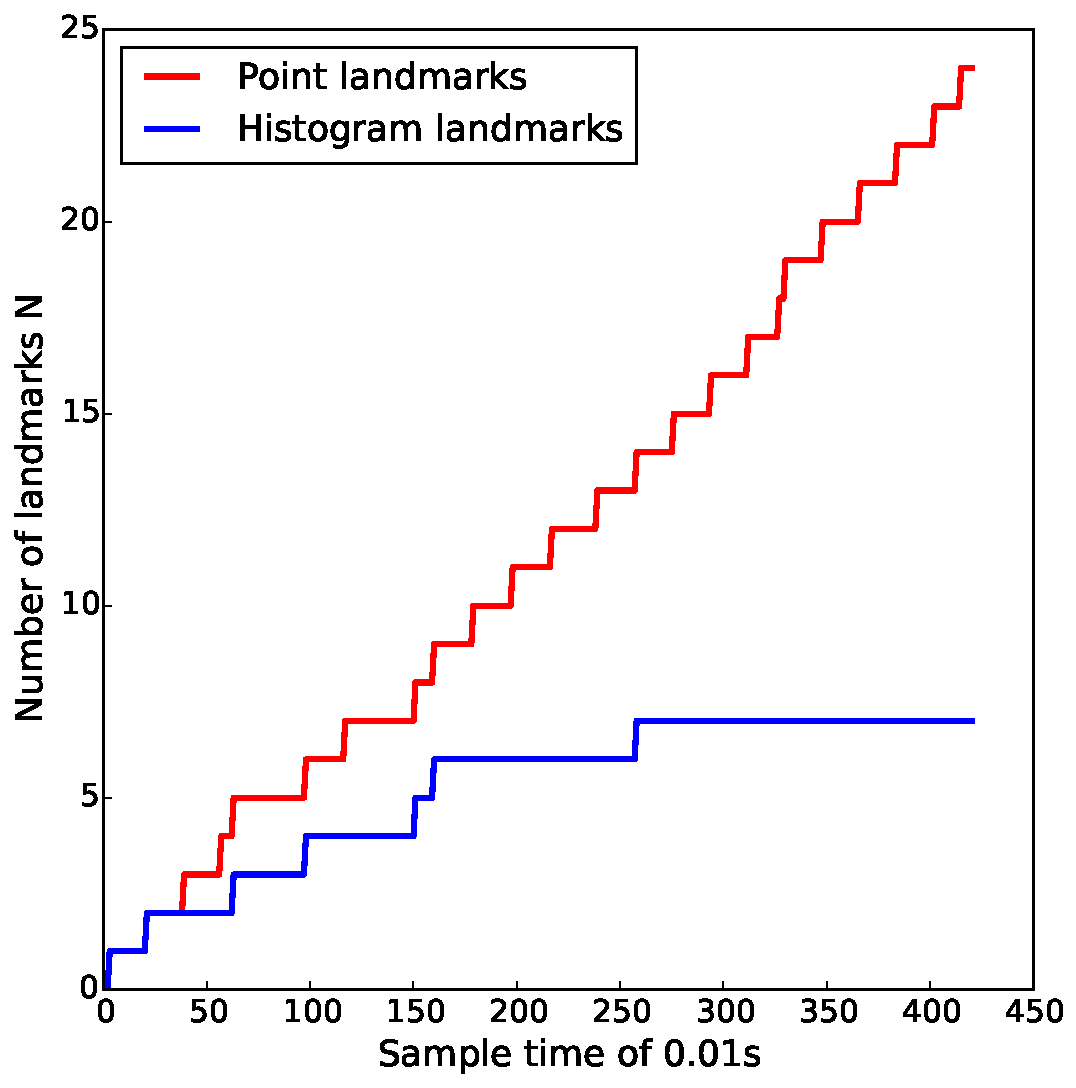
\includegraphics[scale=0.5]{./images/num_landmark}
\caption[Growth of landmarks for different landmark representations]{Landmark growth for the sample world}
\label{num_landmark}
\end{figure}

The point landmarks case has a diverging SLAM solution since the robot pose error grows with time. The error covariances of the landmarks remain the same since there are no updates. The histogram map rather has a converging solution to the SLAM problem with each covariance of initialized landmark reducing with time, and is bounded since the covariance cannot get lower than the initial covariance of the robot pose \cite{dissanayake2001solution}. The convergence in the landmark estimates for histogram maps, and the map as a whole, is illustrated in Figure~\ref{cov_red}. As the SLAM system is observable and correlated, the SLAM solution converges to a true estimate as well.
\begin{figure}
\centering
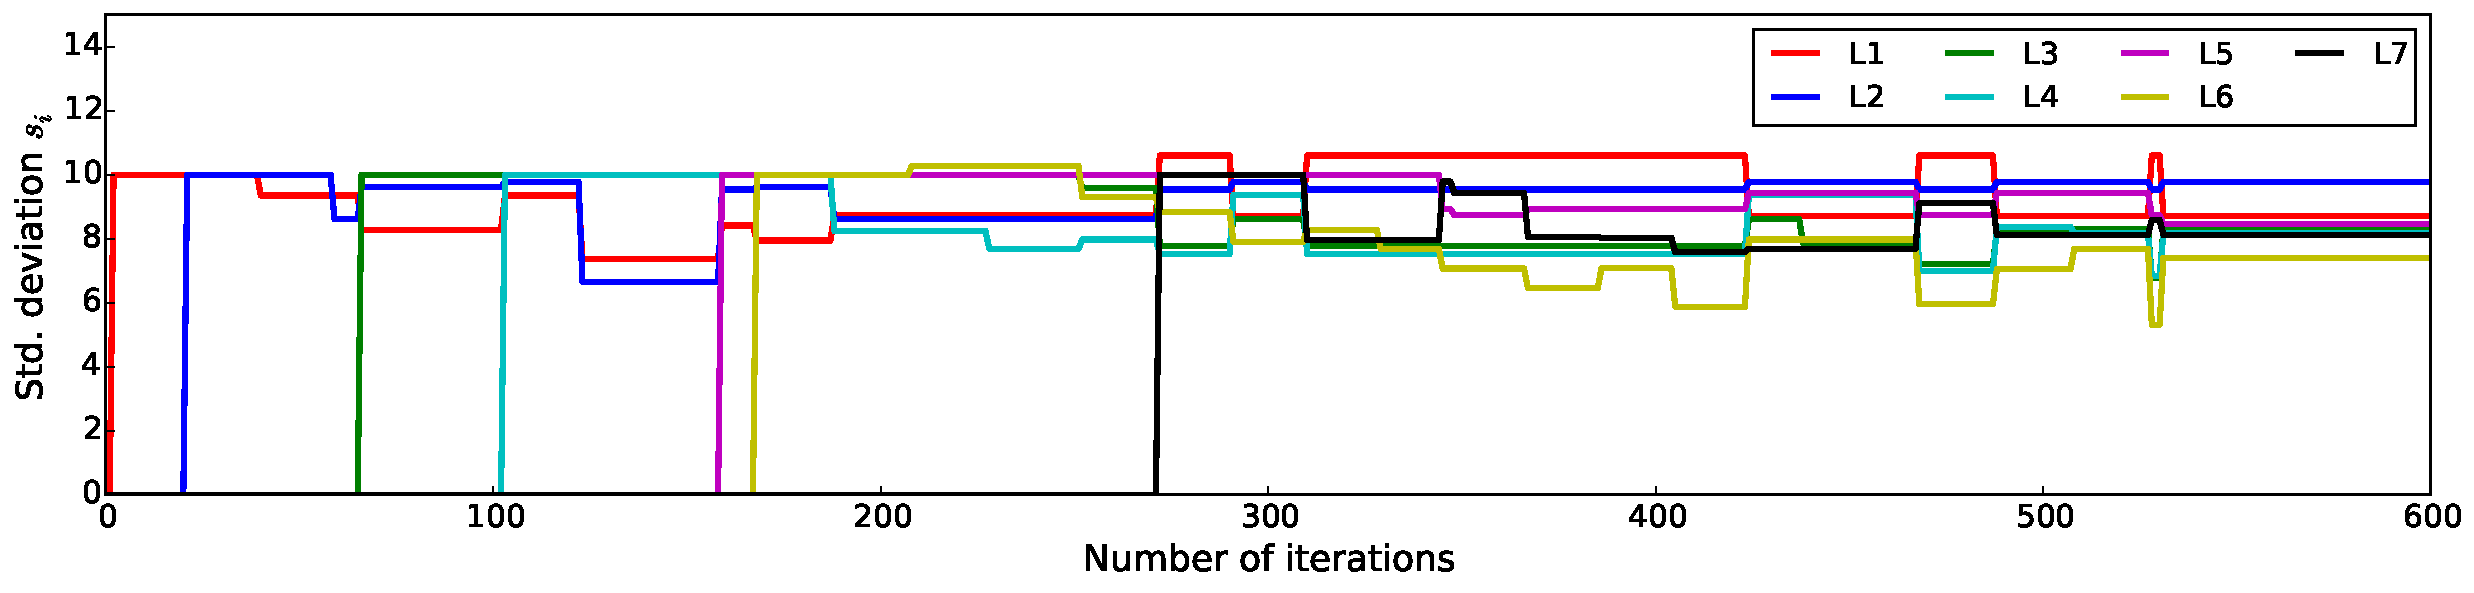
\includegraphics[width=\textwidth]{./images/cov_wc22}
\caption[Convergence rate for different landmarks]{Convergence in landmark uncertainty, and as a result, the convergence of the map. A time history of standard deviations for a set of landmark locations are given where each landmark is initialized with a constant conservative estimate.}
\label{cov_red}
\end{figure} 

The incorporation of indoor geometric constraints such as orthogonality, equal corridor width, etc., can result in a consistent SLAM estimation as showed in Section~\ref{sec::conscorr}. The constraints are incorporated into the EKF-update step as low (close to zero) uncertainty measurements \cite{newman1999structure}. Addition of this geometric update results in a more consistent estimate of landmarks and this update is carried out for every new landmark creation (for a non-zero landmark set) and loop closure. The constraints are established only between neighbouring landmarks. The convergence of the landmark estimates are shown in Figure~\ref{cov_red2}.
 
\begin{figure}
\centering
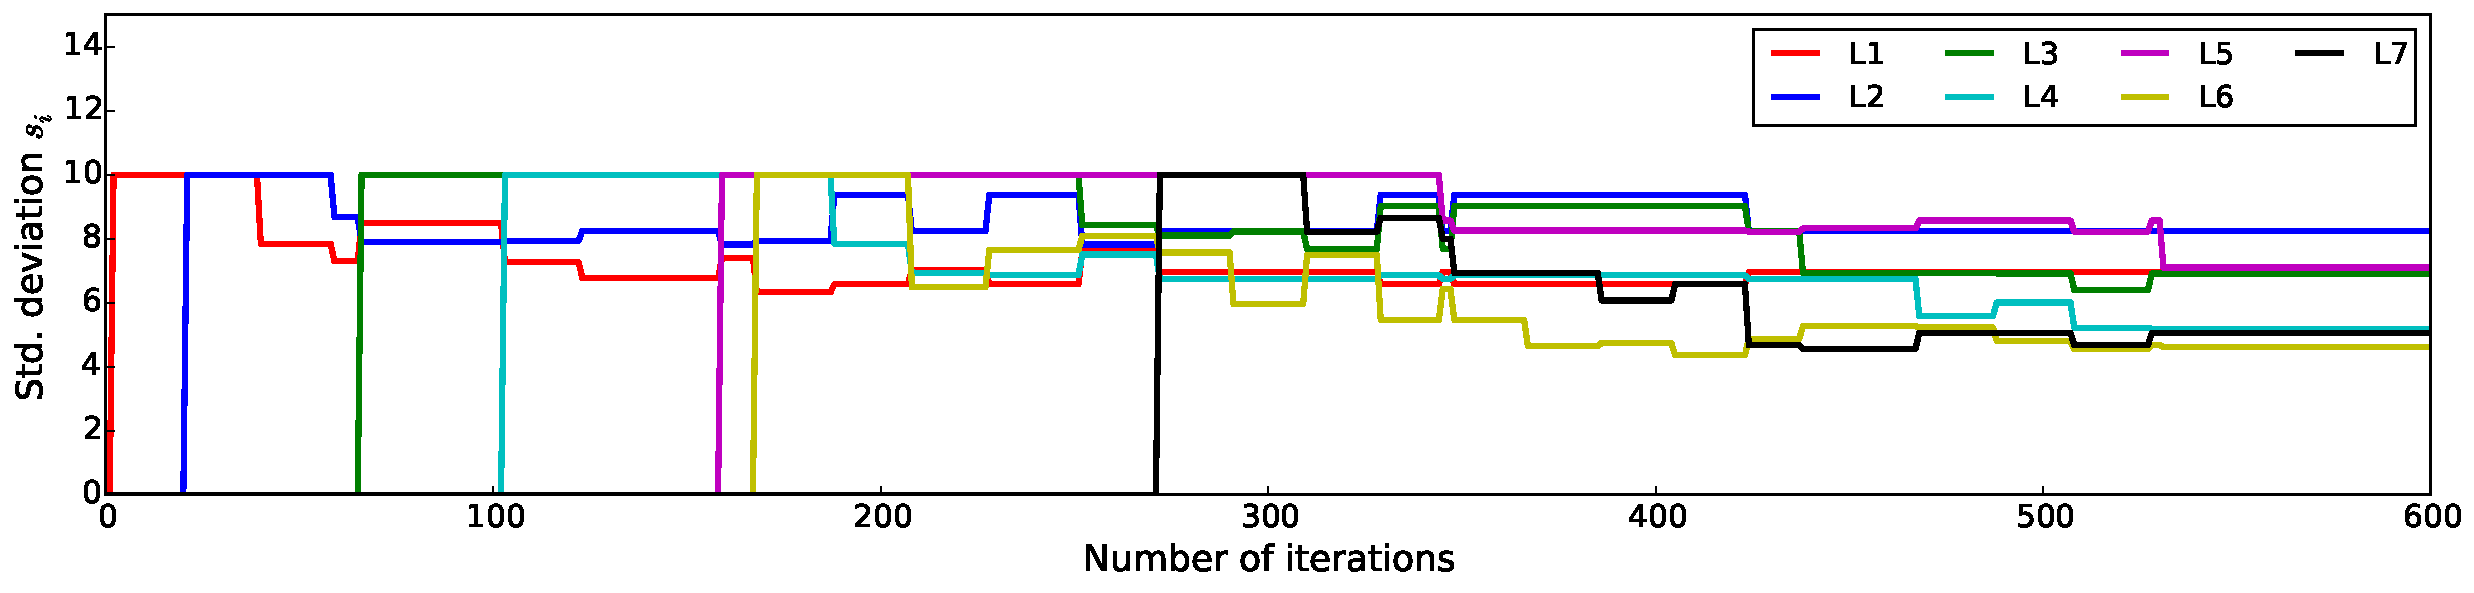
\includegraphics[width=\textwidth]{./images/cov_wc21}
\caption[Increase in convergence rate through addition of rectilinear constraints]{Convergence in landmark uncertainty on incorporation of additional EKF-update using rectilinear geometric constraints. Each landmark is initialized with a conservative covariance estimate.}
\label{cov_red2}
\end{figure}

Additional data processing steps are added to output a good consistent map. The histogram data is propagated using a discrete Bayes filter and the data is compared at every update step to a threshold for a consistent data recording since the histogram is propagated as a probability distribution. The old measurements get discounted slowly due to normalization of the distribution which makes the histogram lose past information. As a result, a simple data processing step is used. Figures~\ref{hist_coll},~\ref{hist_coll2}~and~\ref{hist_coll3} illustrate the propagation of histogram distribution with additional data processing steps such as data thresholding and clubbing of collision information in a histogram (with minimum door opening assumption). Figure~\ref{hist_map} shows the output histogram map of the environment. Note that figure window constraints (map orientation and position) are incorporated for illustration purposes. For the given environment as well as the real world environment to be used in future, the discretizaton level used is $1/l$ where $l$ is the boundary length. The length can also be set arbitrarily and pruned later. 
\begin{figure}
\centering
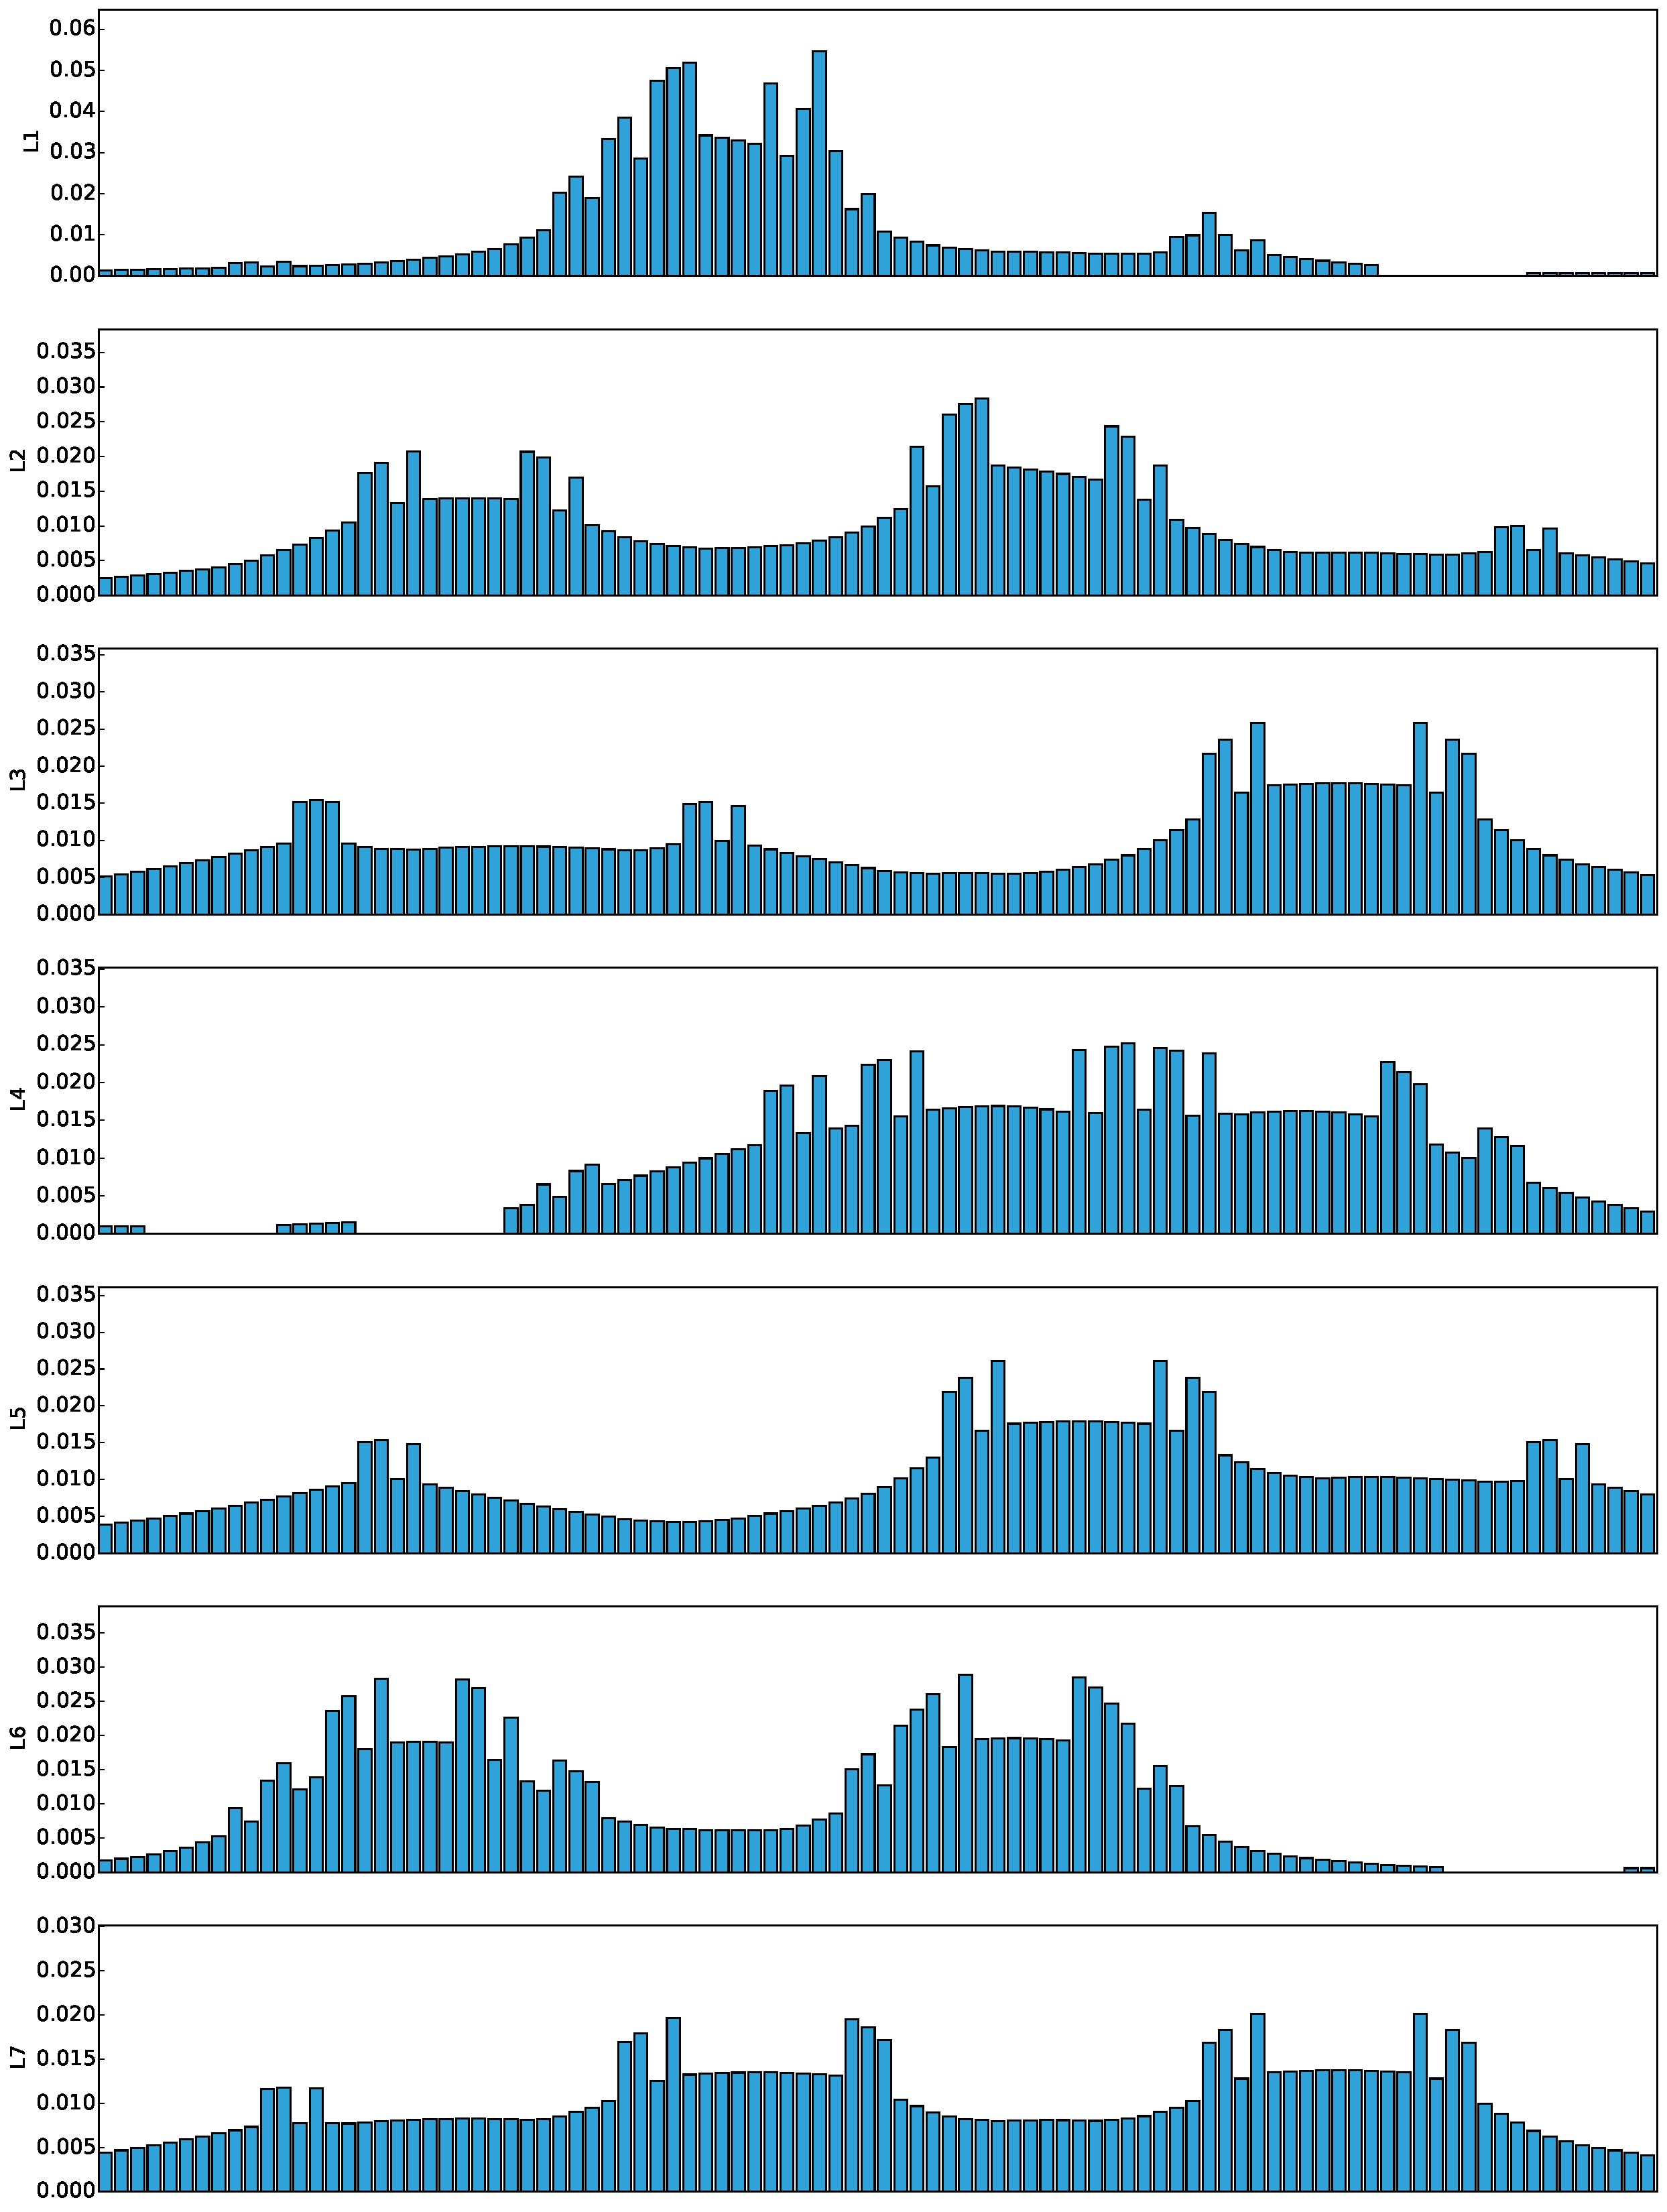
\includegraphics[width=\textwidth]{./images/hist_coll}
\caption[Histogram distribution encoding collision information]{Histogram distribution encoding collision information}
\label{hist_coll}
\end{figure}

\begin{figure}
\centering
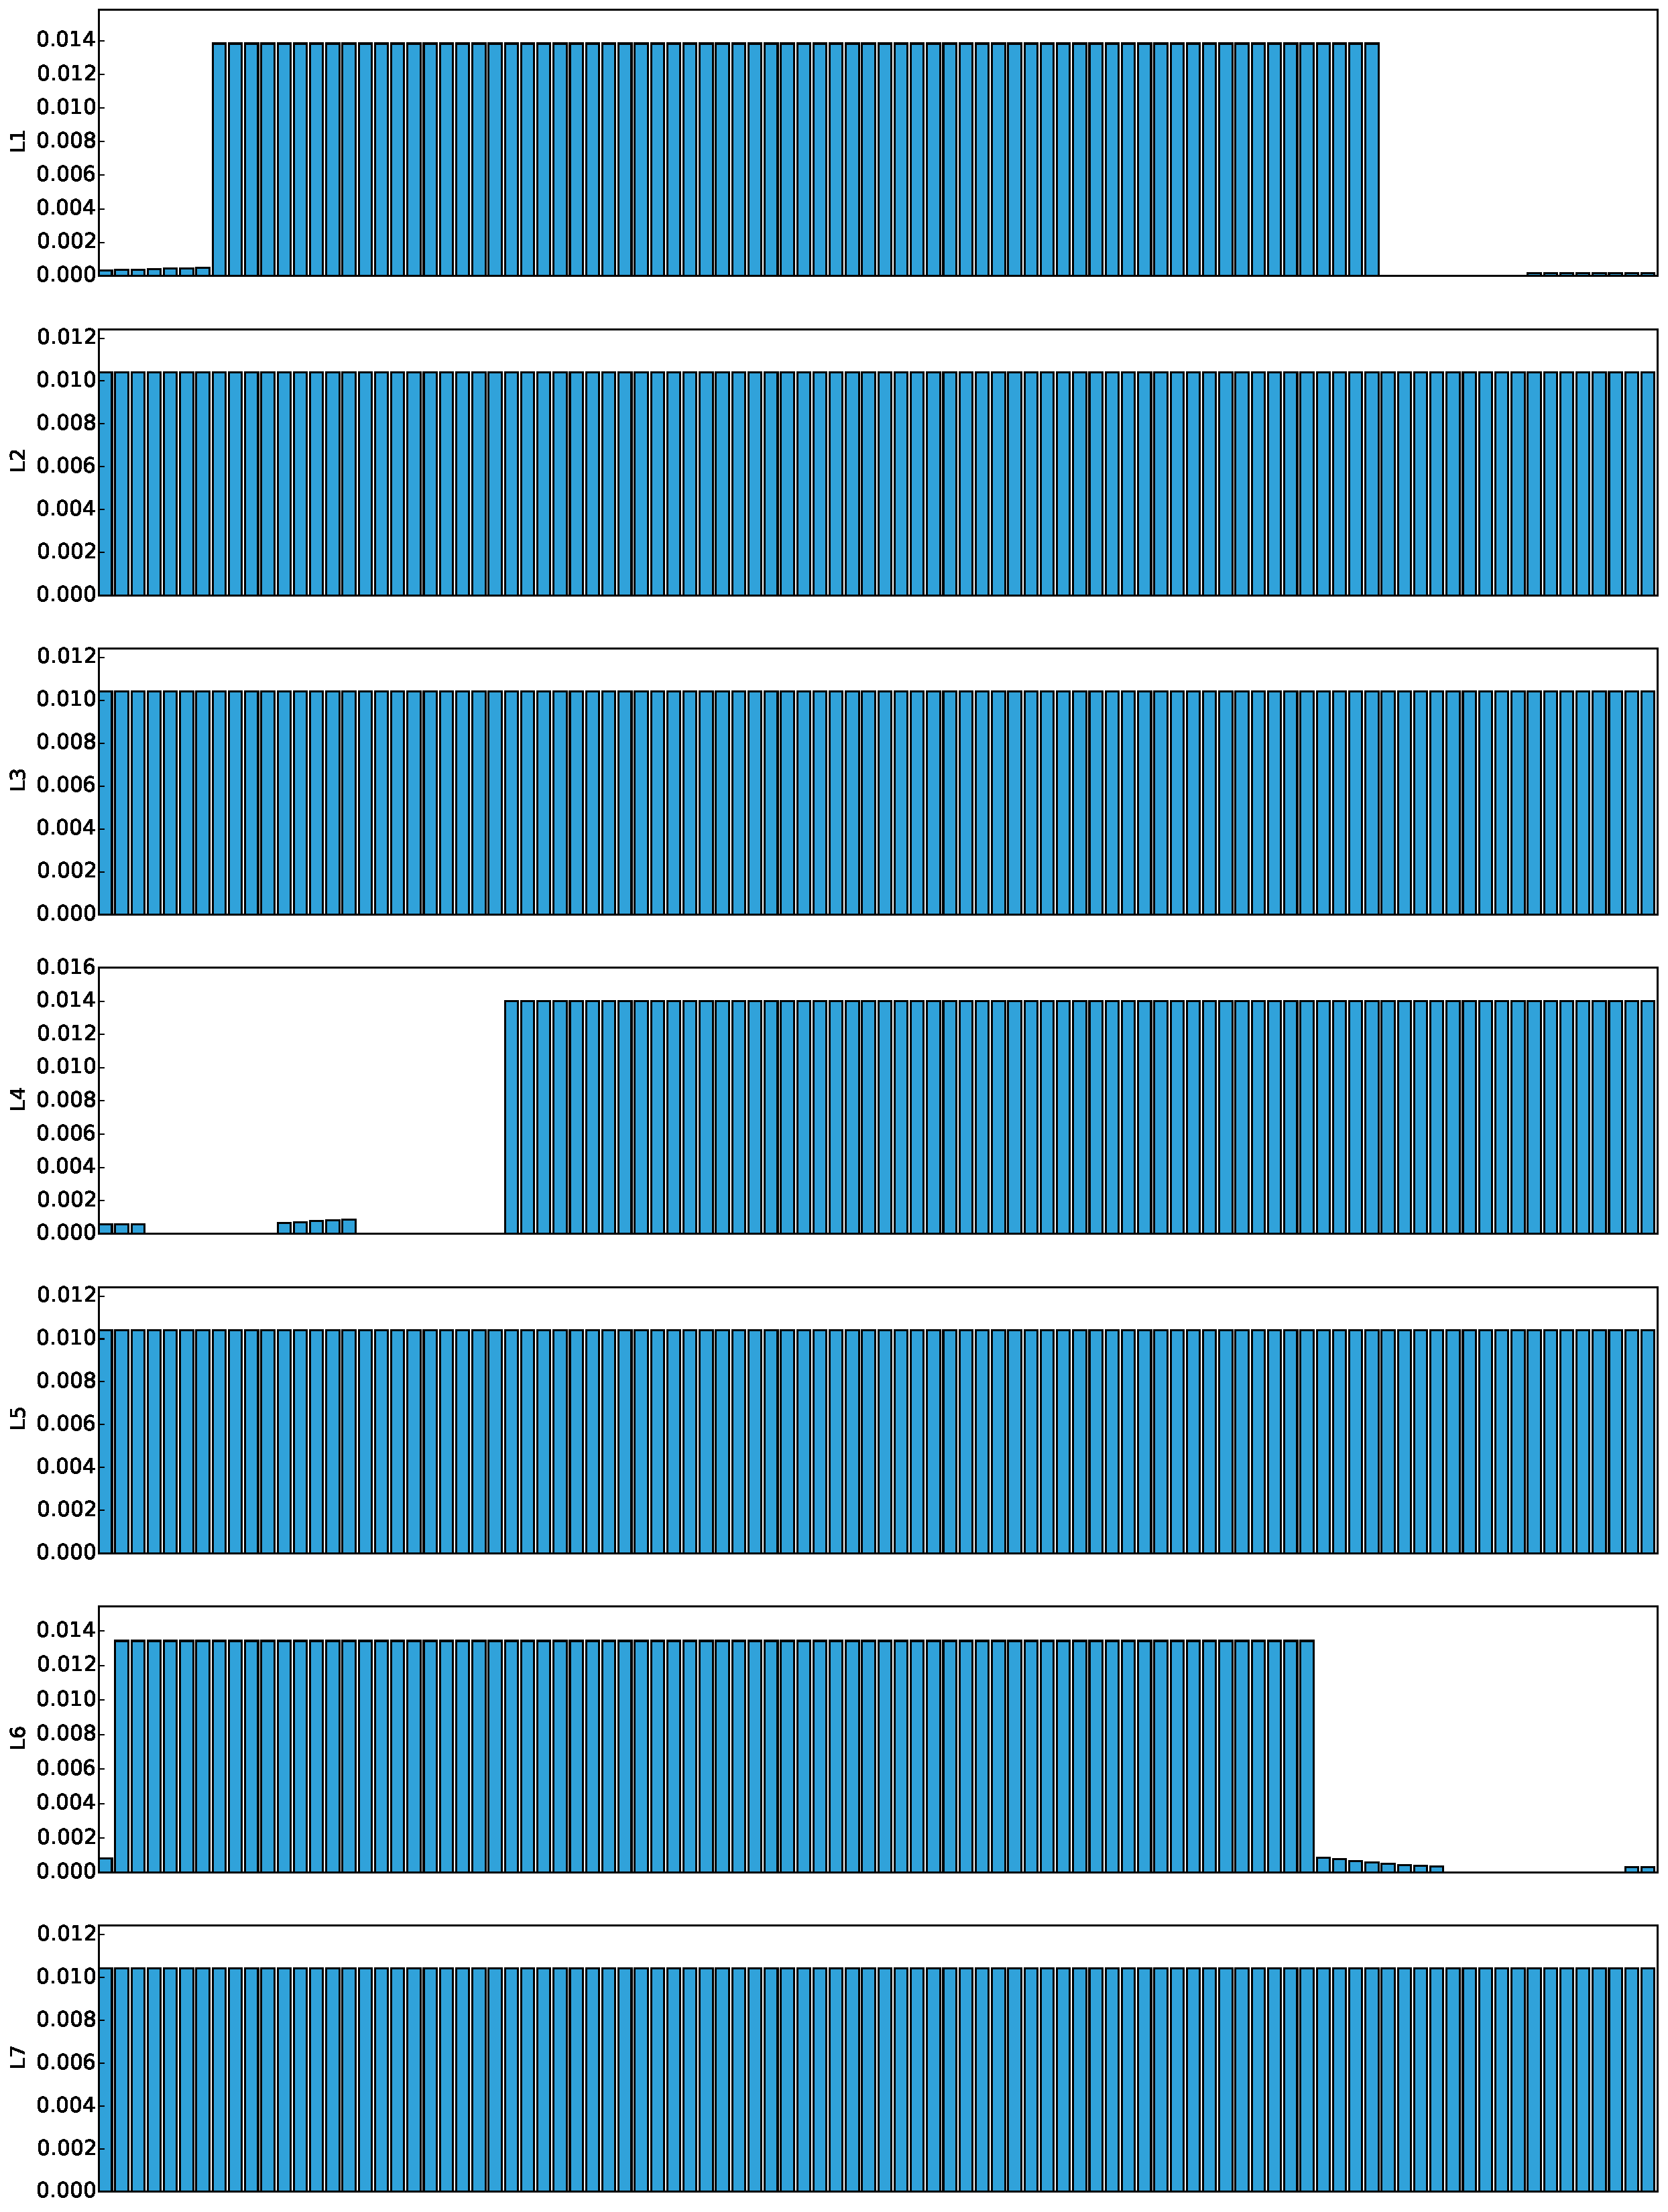
\includegraphics[width=\textwidth]{./images/hist_coll2}
\caption[Processing of the resulting histograms using data threshold]{Processing of the resulting histograms using data threshold}
\label{hist_coll2}
\end{figure}

\begin{figure}
\centering
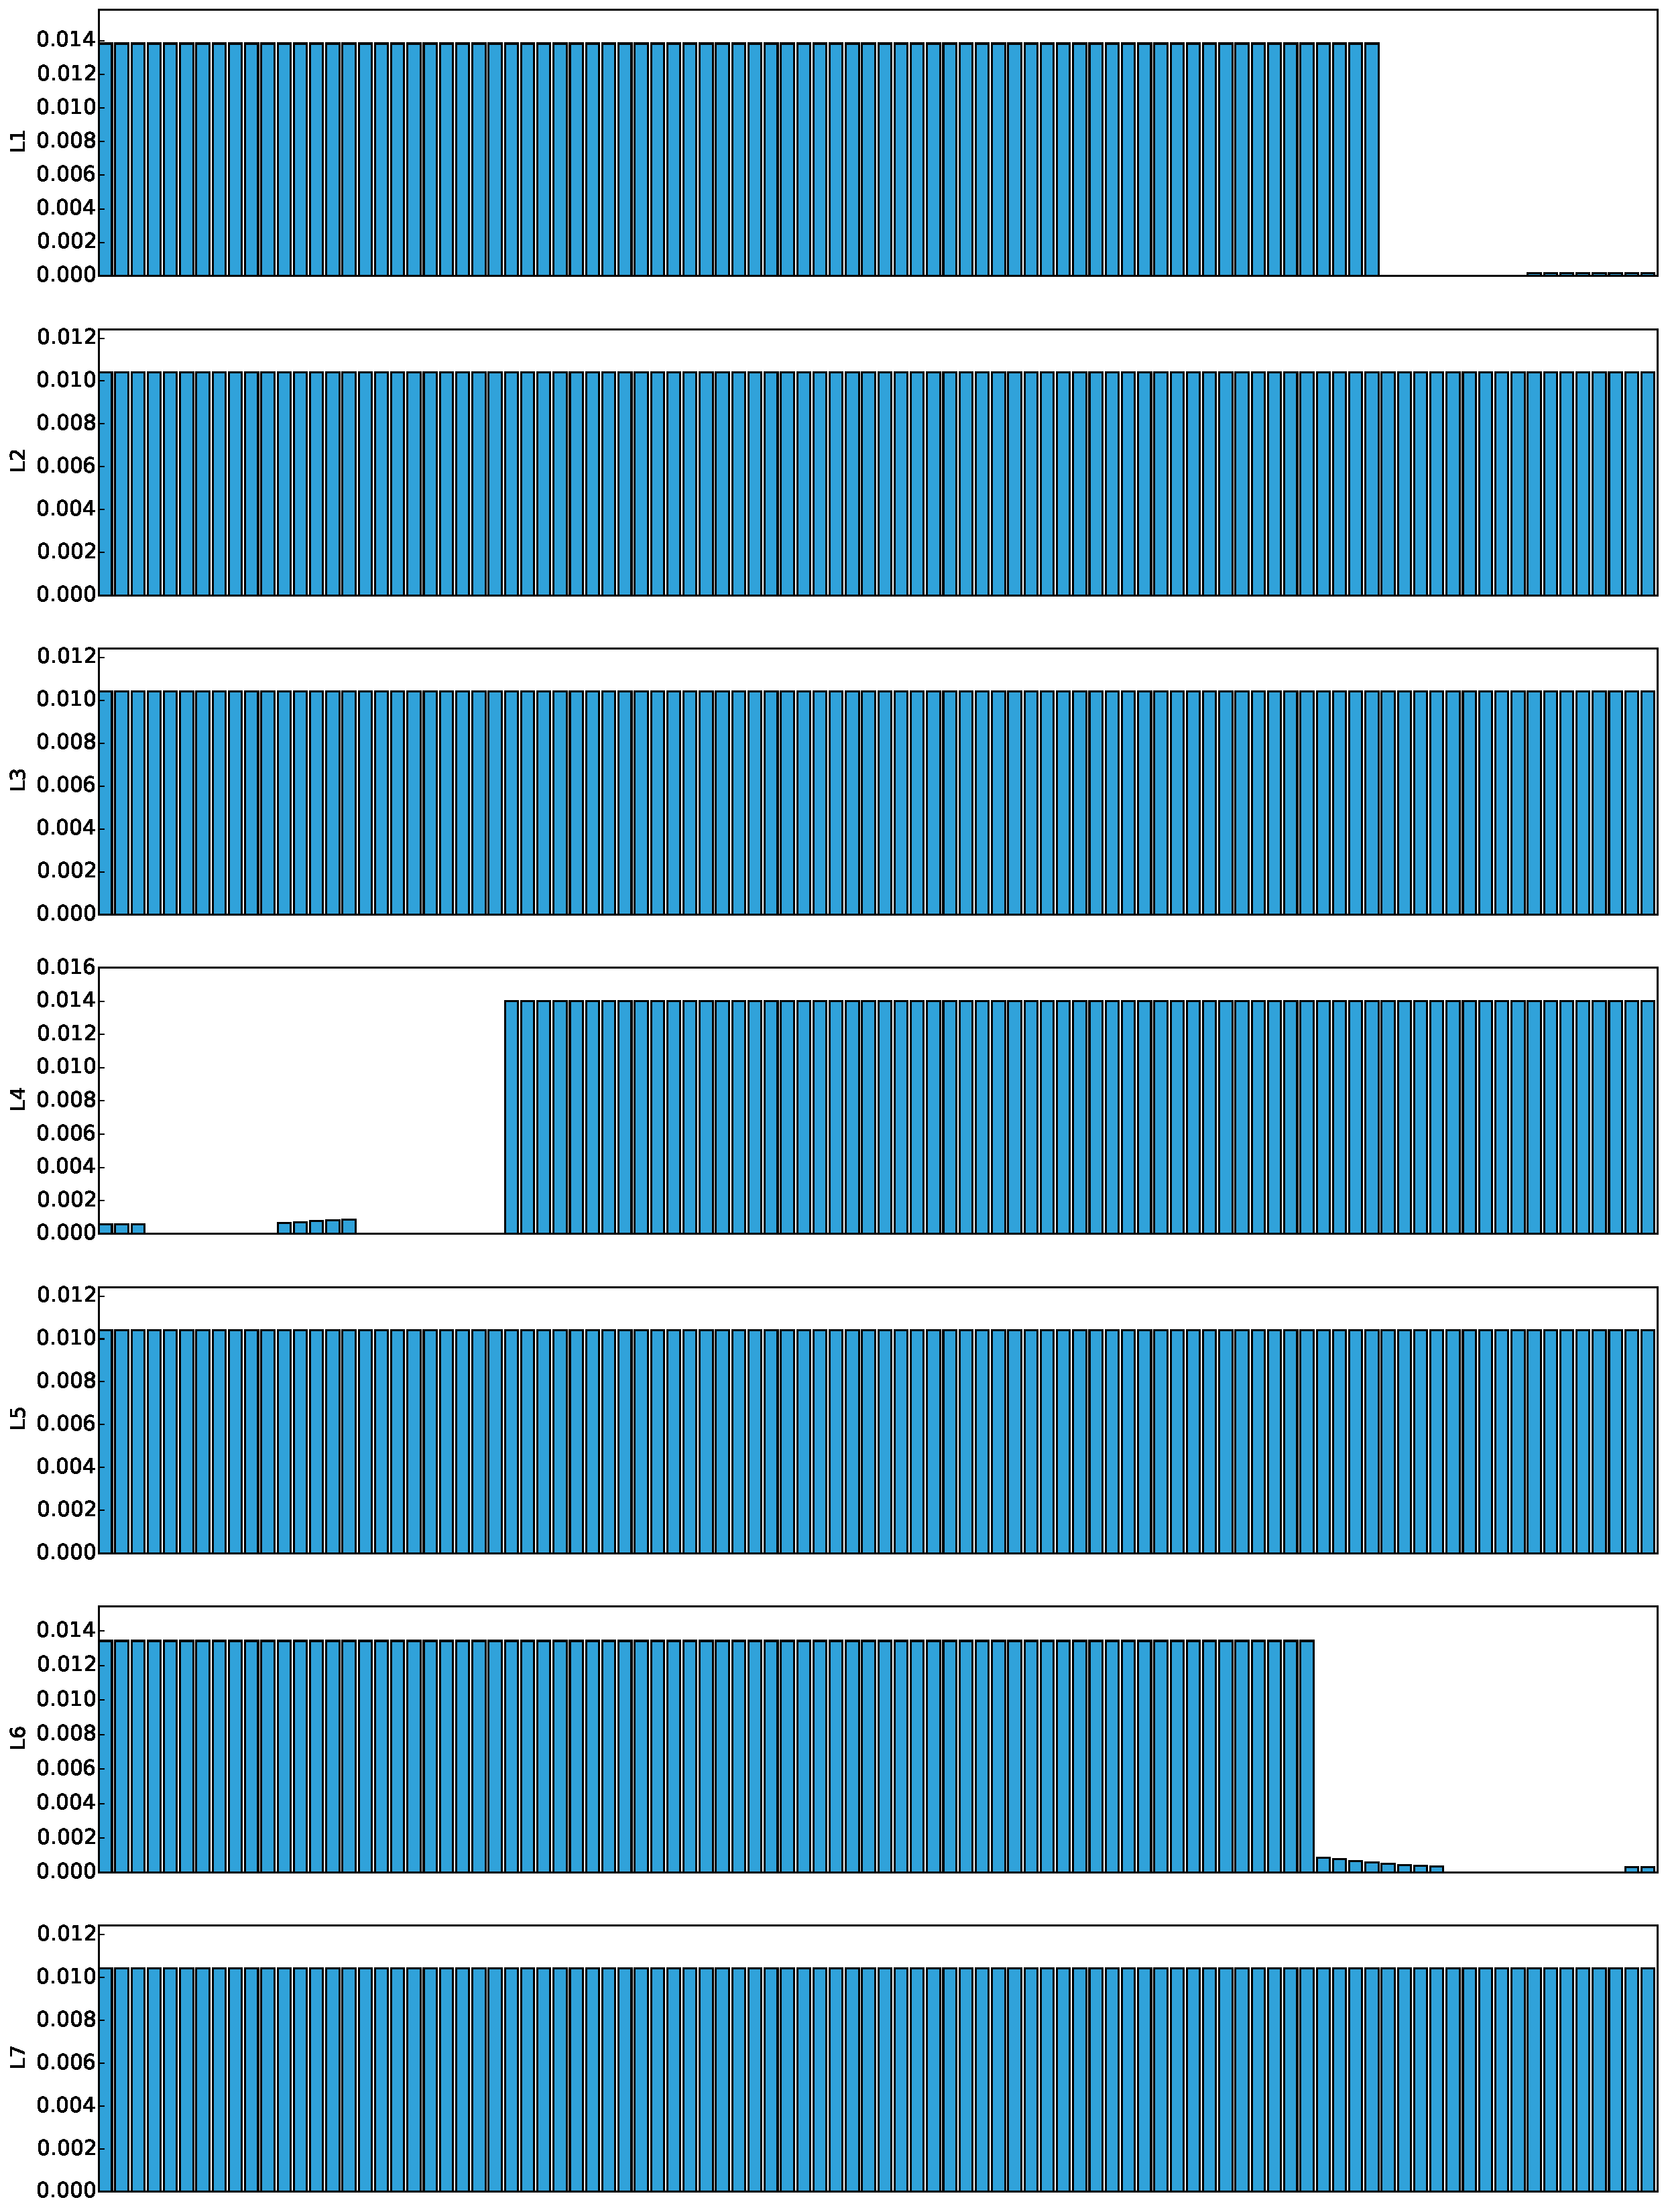
\includegraphics[width=\textwidth]{./images/hist_coll3}
\caption[Clubbing of collision information in the processed histogram]{Clubbing of collision information in the processed histogram}
\label{hist_coll3}
\end{figure}

\begin{figure}
\centering
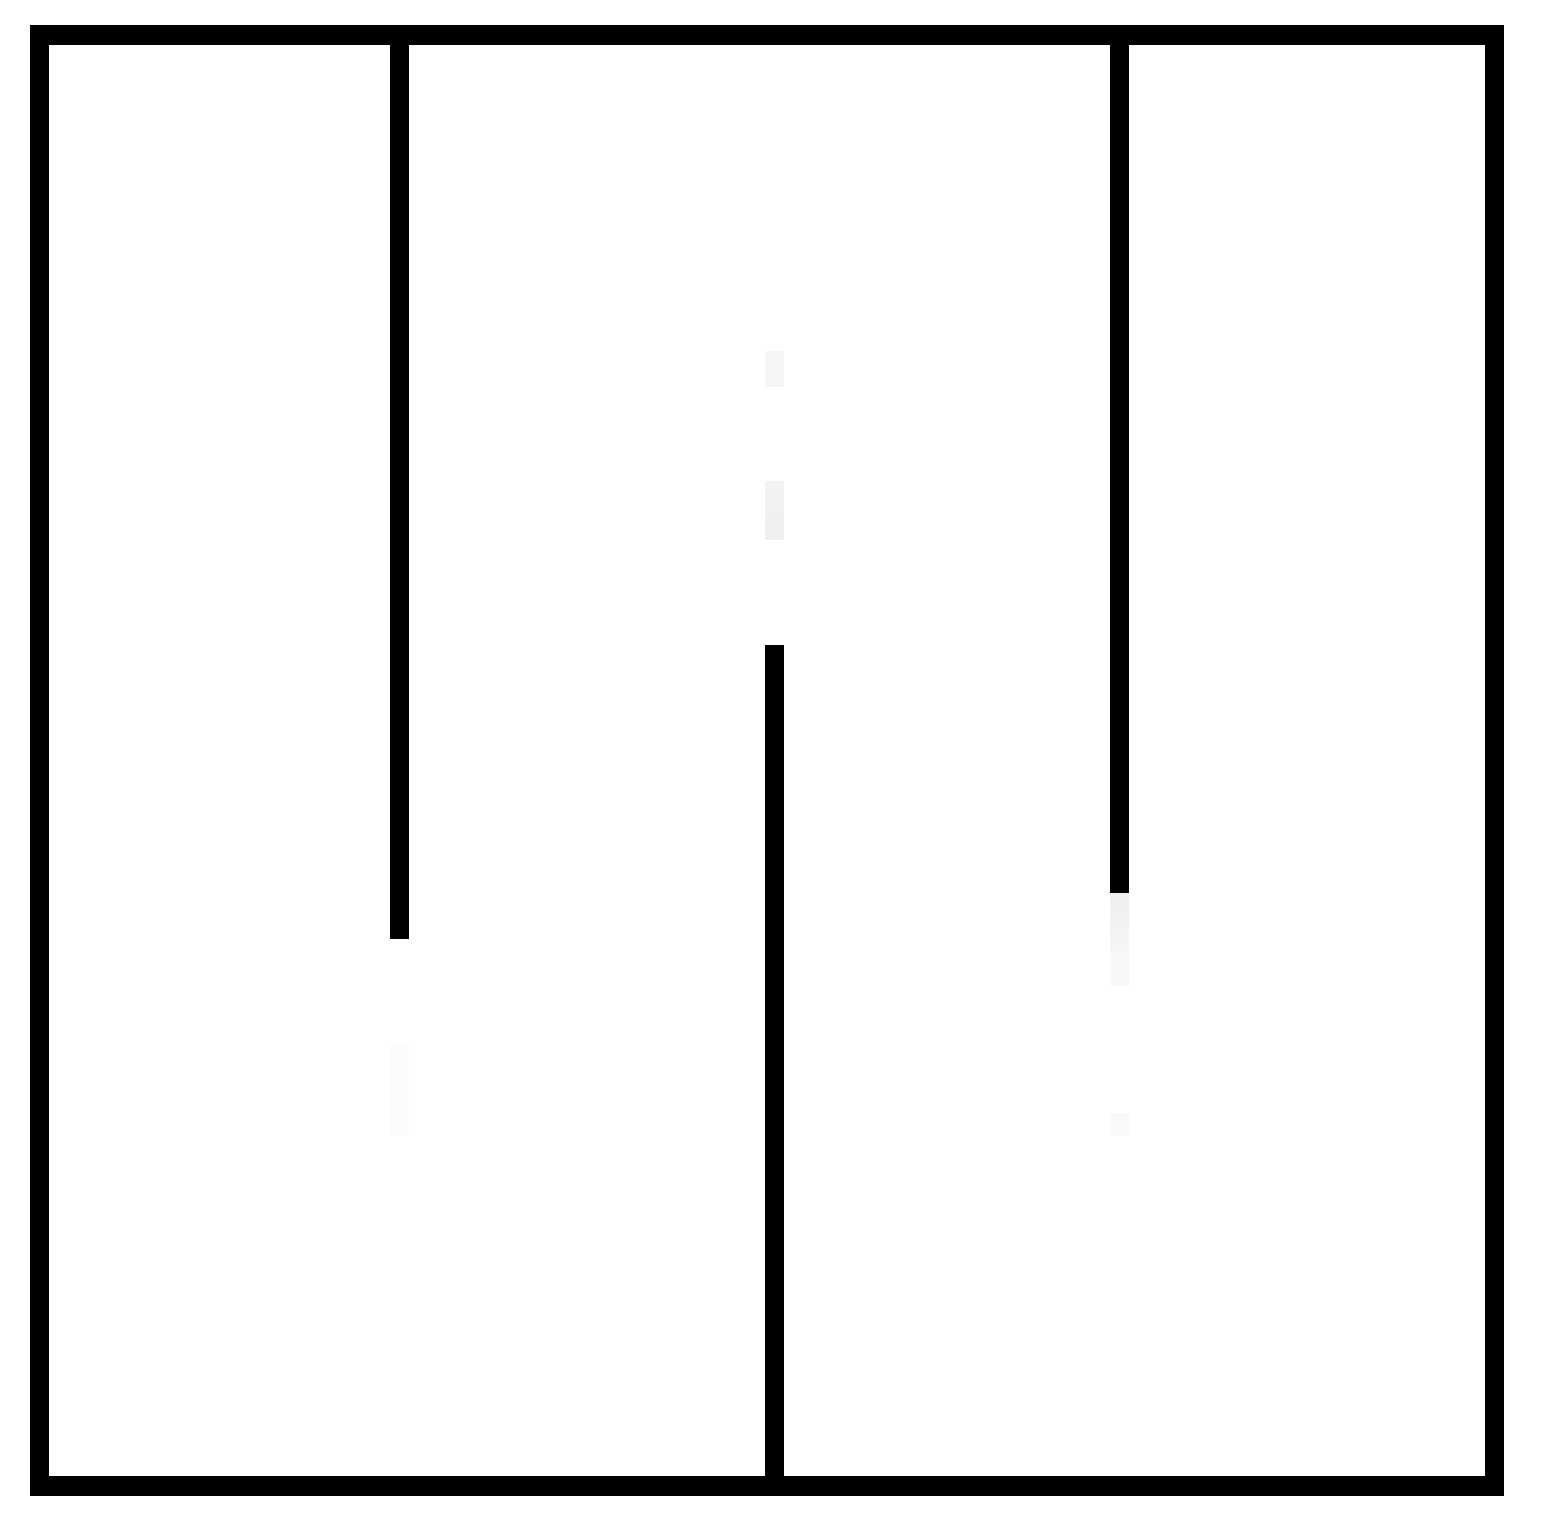
\includegraphics[scale=0.3]{./images/hist_map}
\caption[Output histogram map of the simulated environment]{Histogram map of the sample world for impact-based SLAM}
\label{hist_map}
\end{figure}

Regarding the issue of consistency, there is not much reduction in the particle diversity since the impact-based SLAM does not have dense measurements. Hence, the information provided through the sparse measurements, along with frequent loop closures and indoor constraints provide a good estimate of the particles through the modified proposal. As a result, resampling steps were carried out less frequently with the help of adaptive resampling. For situations involving large indoor environments, the frequency of resampling might increase due to the accumulated noise over the measurements which can lead to inconsistency.

A long term inconsistency through resampling can be avoided using multiple robots exploring the environment. The multiple robot scenario can occur in two ways, either robots collect measurements for a period of time and commonly (centralized processing) implement SLAM or the individual robots do a separate SLAM and merge the local maps at a later time. The later approach will be adopted in this thesis.

The maps collected by the individual robots are merged using a simple map comparison with consideration of additional assumptions. The assumptions considered are environment size and approximate starting points for the robot. The multiple robot reduces the exploration time and at the same time improving the local consistency of the solution.

In the simulation, the robots start at the corners of the maze which helps in restricting the possibilities of map comparisons. The robots start to do impact-based SLAM separately and no communication is present between the robots. The robots communicate to a central processing unit where the map merging occurs. The individual maps are merged together once a similarity between the individual maps is found. The merged map generated using two robots are shown in Figure~\ref{merge_map}. 

\begin{rem}
The multiple robot SLAM discussed in this thesis is not a distributed SLAM problem since the merged map does not influence the particle poses of each robot.
\end{rem}

The similarity between the individual maps are found through finite comparisons of histograms. The finite nature of comparisons is attributed due to geometric considerations in the environment that were used for pruning possibilities in the data association along with the additional assumptions.
\begin{figure}
\centering
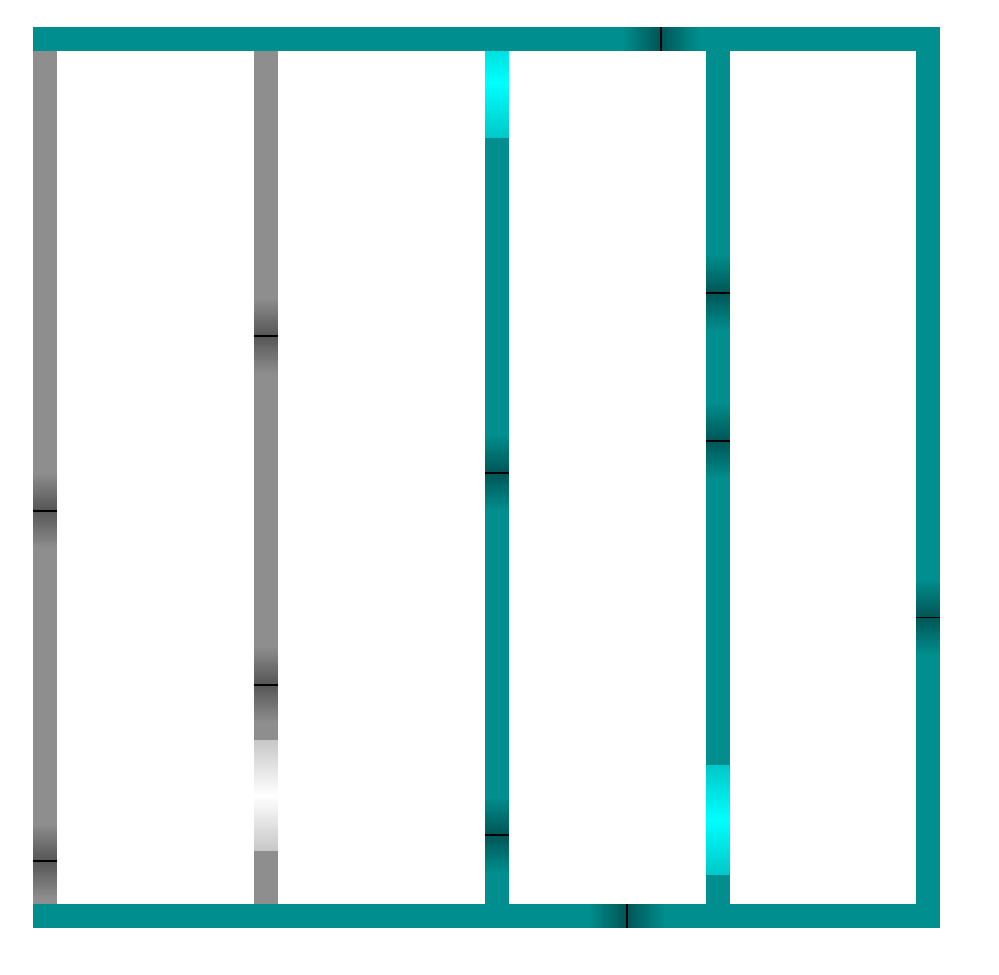
\includegraphics[scale=0.6]{./images/merge_map}
\caption[Merged map of the sample environment using two robots]{Merged map of the sample environment using two robots. Map of robot 1 is shown in gray scale while map of robot 2 is shown in cyan scale.}
\label{merge_map}
\end{figure} 

\textbf{Summary}
In this chapter, a detailed algorithm of particle filter-SLAM is provided with the key steps detailed with algorithms and figures. A flowchart is illustrated for clarity of the algorithm. Examples are provided to get an understanding of the landmark initialization and updates for a histogram map. Simulation results are analyzed and issues such as convergence and consistency are addressed.